\documentclass[UTF8]{ctexbeamer}

\usetheme{Boadilla}
\usefonttheme[onlymath]{serif}

% Title
\title{第2章 建模过程、比例性和几何相似性}
\author{韩建伟}
\institute{
  计算机学院\\
  \texttt{hanjianwei@zjgsu.edu.cn}
}
\date{2018/10/12}

\begin{document}

% Title page
\begin{frame}[plain]
  \titlepage{}
\end{frame}

\begin{frame}{现实世界与数学世界}

  \begin{center}
    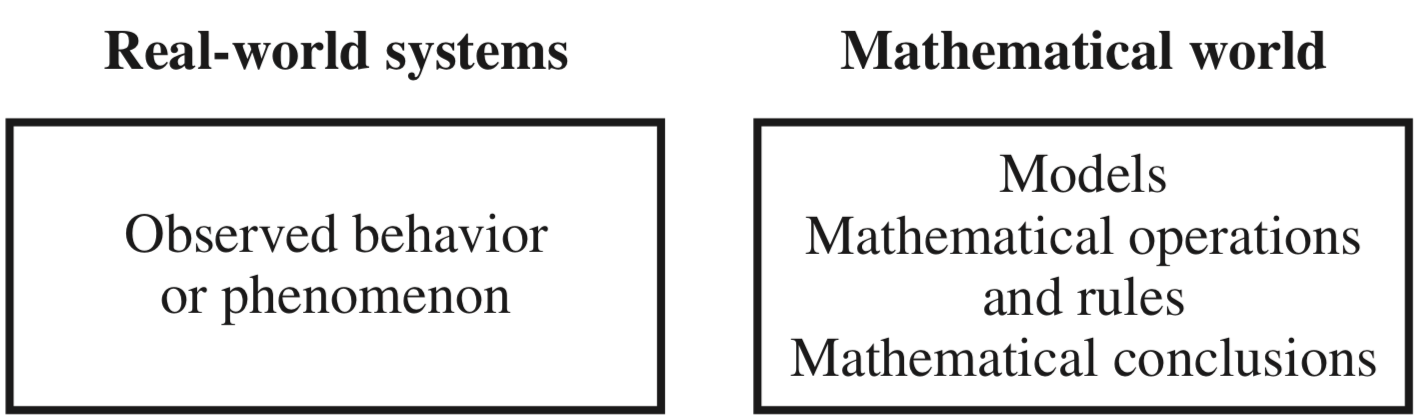
\includegraphics[width=.5\textwidth{}]{real_and_math.png}
  \end{center}

  构建模型来了解世界

  \begin{itemize}
  \item 对现实世界的行为或现象的未来进行预测,分析各种行为对其影响
  \item 系统: 一些有规律的相互作用或内在的依赖关系联结在一起的对象集合体
  \item 建模者希望了解一个特殊的系统是怎么工作的
  \item 是什么造成了系统变化系统对某些变化有多敏感
  \item 预测系统变化以及何时发生变化
  \end{itemize}

\end{frame}

\begin{frame}{为什么要建模}
  \begin{center}
    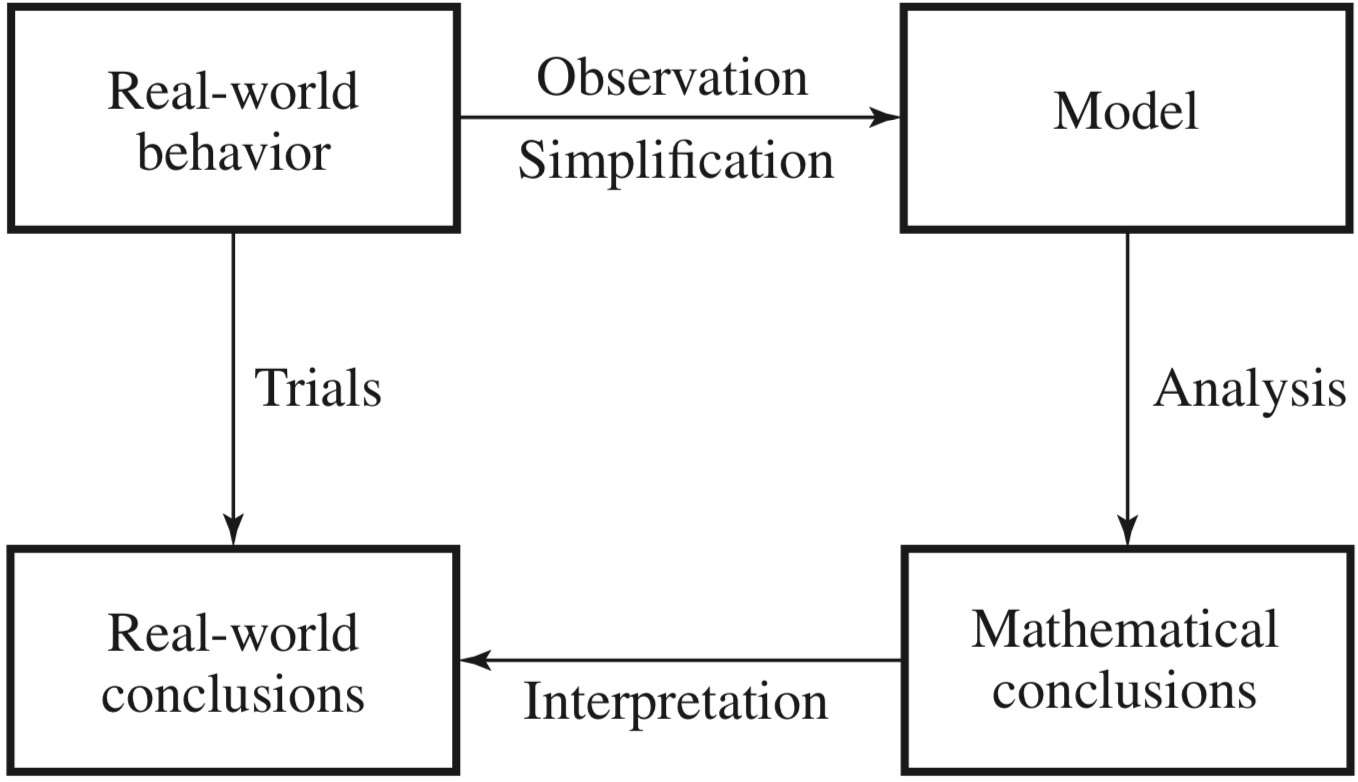
\includegraphics[width=.5\textwidth{}]{whymm.png}
  \end{center}

  \begin{itemize}
  \item 直接进行试验成本很高
  \end{itemize}
\end{frame}

\begin{frame}{建模的步骤}

  \begin{enumerate}
  \item 通过观察,识别有关实际行为的主要因素,可能要做简化
  \item 猜测因素之间暂时的关系
  \item 将数学分析用于所得到的模型
  \item 借助实际问题来解释数学的结论
  \end{enumerate}

  \begin{center}
    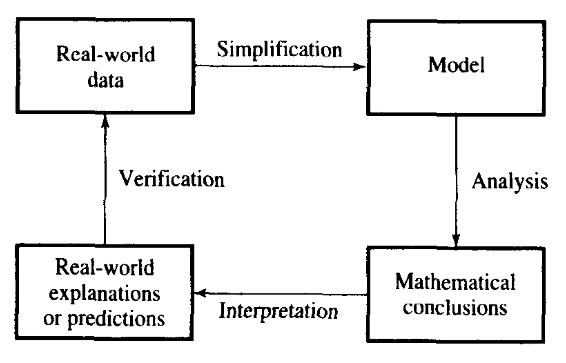
\includegraphics[width=.5\textwidth{}]{mmstep.png}
  \end{center}
\end{frame}

\begin{frame}{数学模型}

  \begin{block}{定义}
    为了研究特定的实际系统或现象而设计的数学结构,图示、符号、模拟和实验结构都包括在内.
  \end{block}

  \begin{center}
    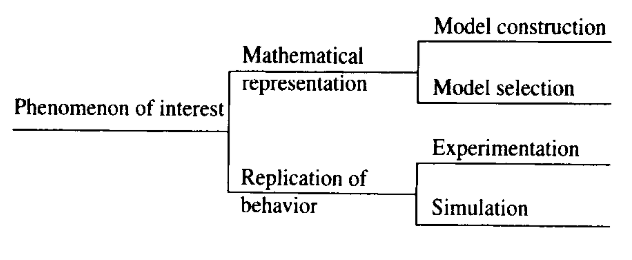
\includegraphics[width=.6\textwidth{}]{modelprop.png}
  \end{center}
  
\end{frame}

\begin{frame}{模型的性质}
  \begin{description}
  \item[保真性] 模型表示现实的精确性
  \item[成本] 建模过程的总费用
  \item[灵活性] 当收集到了所需要的数据时,改变和控制影响改模型的诸多条件的能力
  \end{description}
  
  \begin{center}
    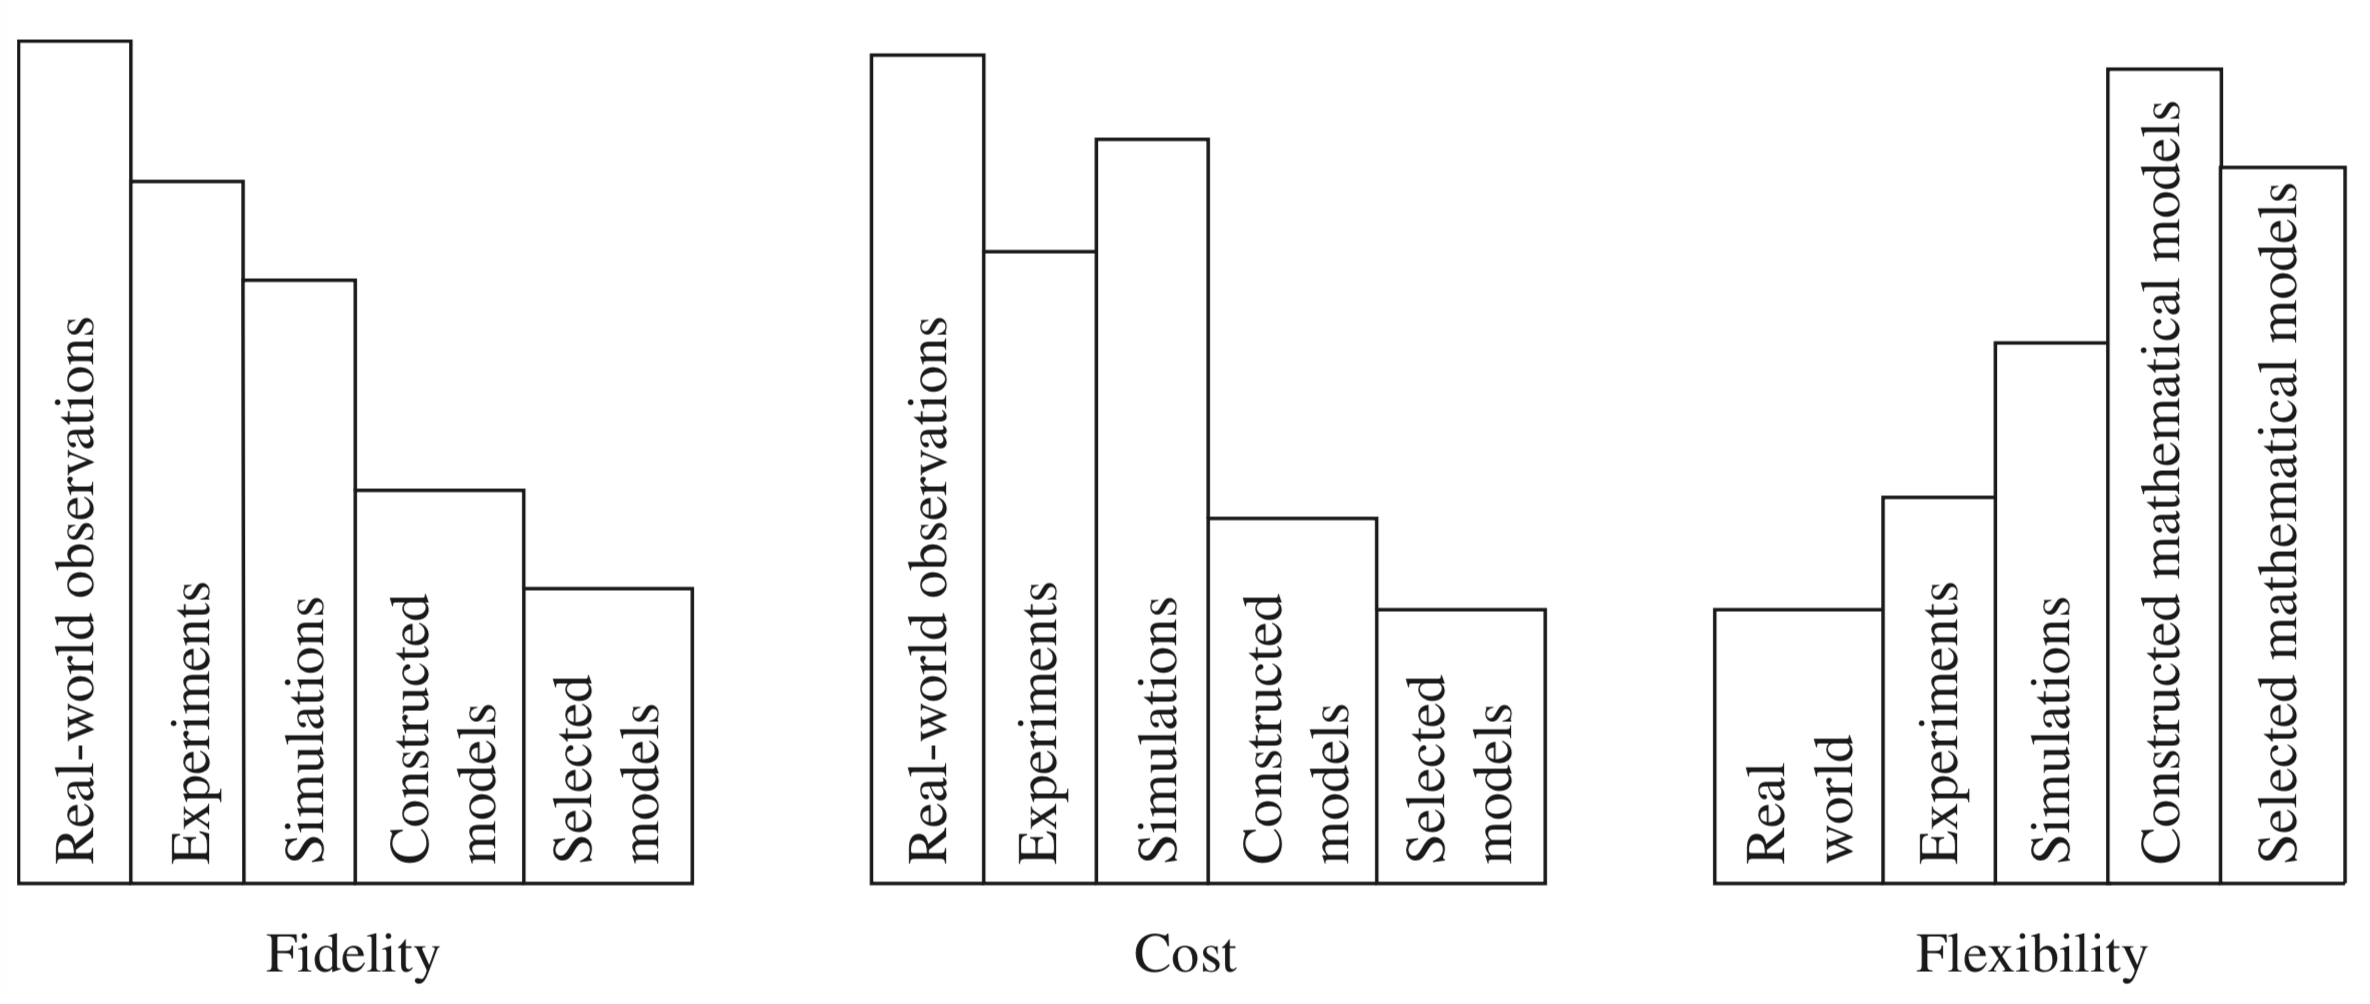
\includegraphics[width=.6\textwidth{}]{modelcompare.png}
  \end{center}
\end{frame}

\begin{frame}{模型的构建}

  \begin{enumerate}
  \item 识别问题
  \item 做出假设
    \begin{enumerate}
    \item 识别变量并对变量进行分类
    \item 确定研究中所选择的变量和子模型之间的相互关系
    \end{enumerate}
  \item 求解或解释模型
  \item 验证模型
    \begin{enumerate}
    \item 表述了问题吗?
    \item 在通常的意义下它有意义吗?
    \item 用实际数据来检验该模型
    \end{enumerate}
  \item 实施模型
  \item 维修模型
  \end{enumerate}
  
\end{frame}

\begin{frame}{车辆的停止距离}

  \begin{description}
  \item[情景] 车与车之间的跟随距离
    \begin{itemize}
    \item 每10英里的速度允许一辆车长度的跟随距离
    \item 看着前车刚驶过的点, 2秒之内到达表示太近了
    \end{itemize}
  \item[识别问题] 预测作为车辆速率函数的车辆的总的停止距离(跟车距离)
  \item[假设] 总的停止距离 = 反应距离 + 刹车距离
    \begin{itemize}
    \item 反应距离 = $f$(反应时间, 速率)
    \item 刹车距离 = $h$(重量, 速率)
    \end{itemize}
  \item[验证] 不符合实际驾驶情形$\Rightarrow$评估某些假设,或重新构建子模型
  \item[实施] 只有易于理解并易于使用的才是有效的
  \item[维修] 机动刹车或圆盘刹、车胎设计等基本变化
  \end{description}
  
\end{frame}

\begin{frame}{和科学方法的对比}

  \begin{enumerate}
  \item 对现象做一些一般性的观察
  \item 形成关于观察的假设
  \item 研制检验该假设的一种方法
  \item 收集用于改检验的数据
  \item 利用改数据来检验假设
  \item 肯定或者拒绝该假设
  \end{enumerate}

  \begin{description}
  \item[相似之处] 都包括假设、收集实际数据以及用数据来检验或验证假设
  \item[不同之处] 数学建模是假设一个模型,而科学方法是确认模型;数学模型的目标不是肯定或者拒绝该模型,而是检验其合理性
  \end{description}
  
\end{frame}

\begin{frame}{模型的迭代性质}

  \begin{center}
    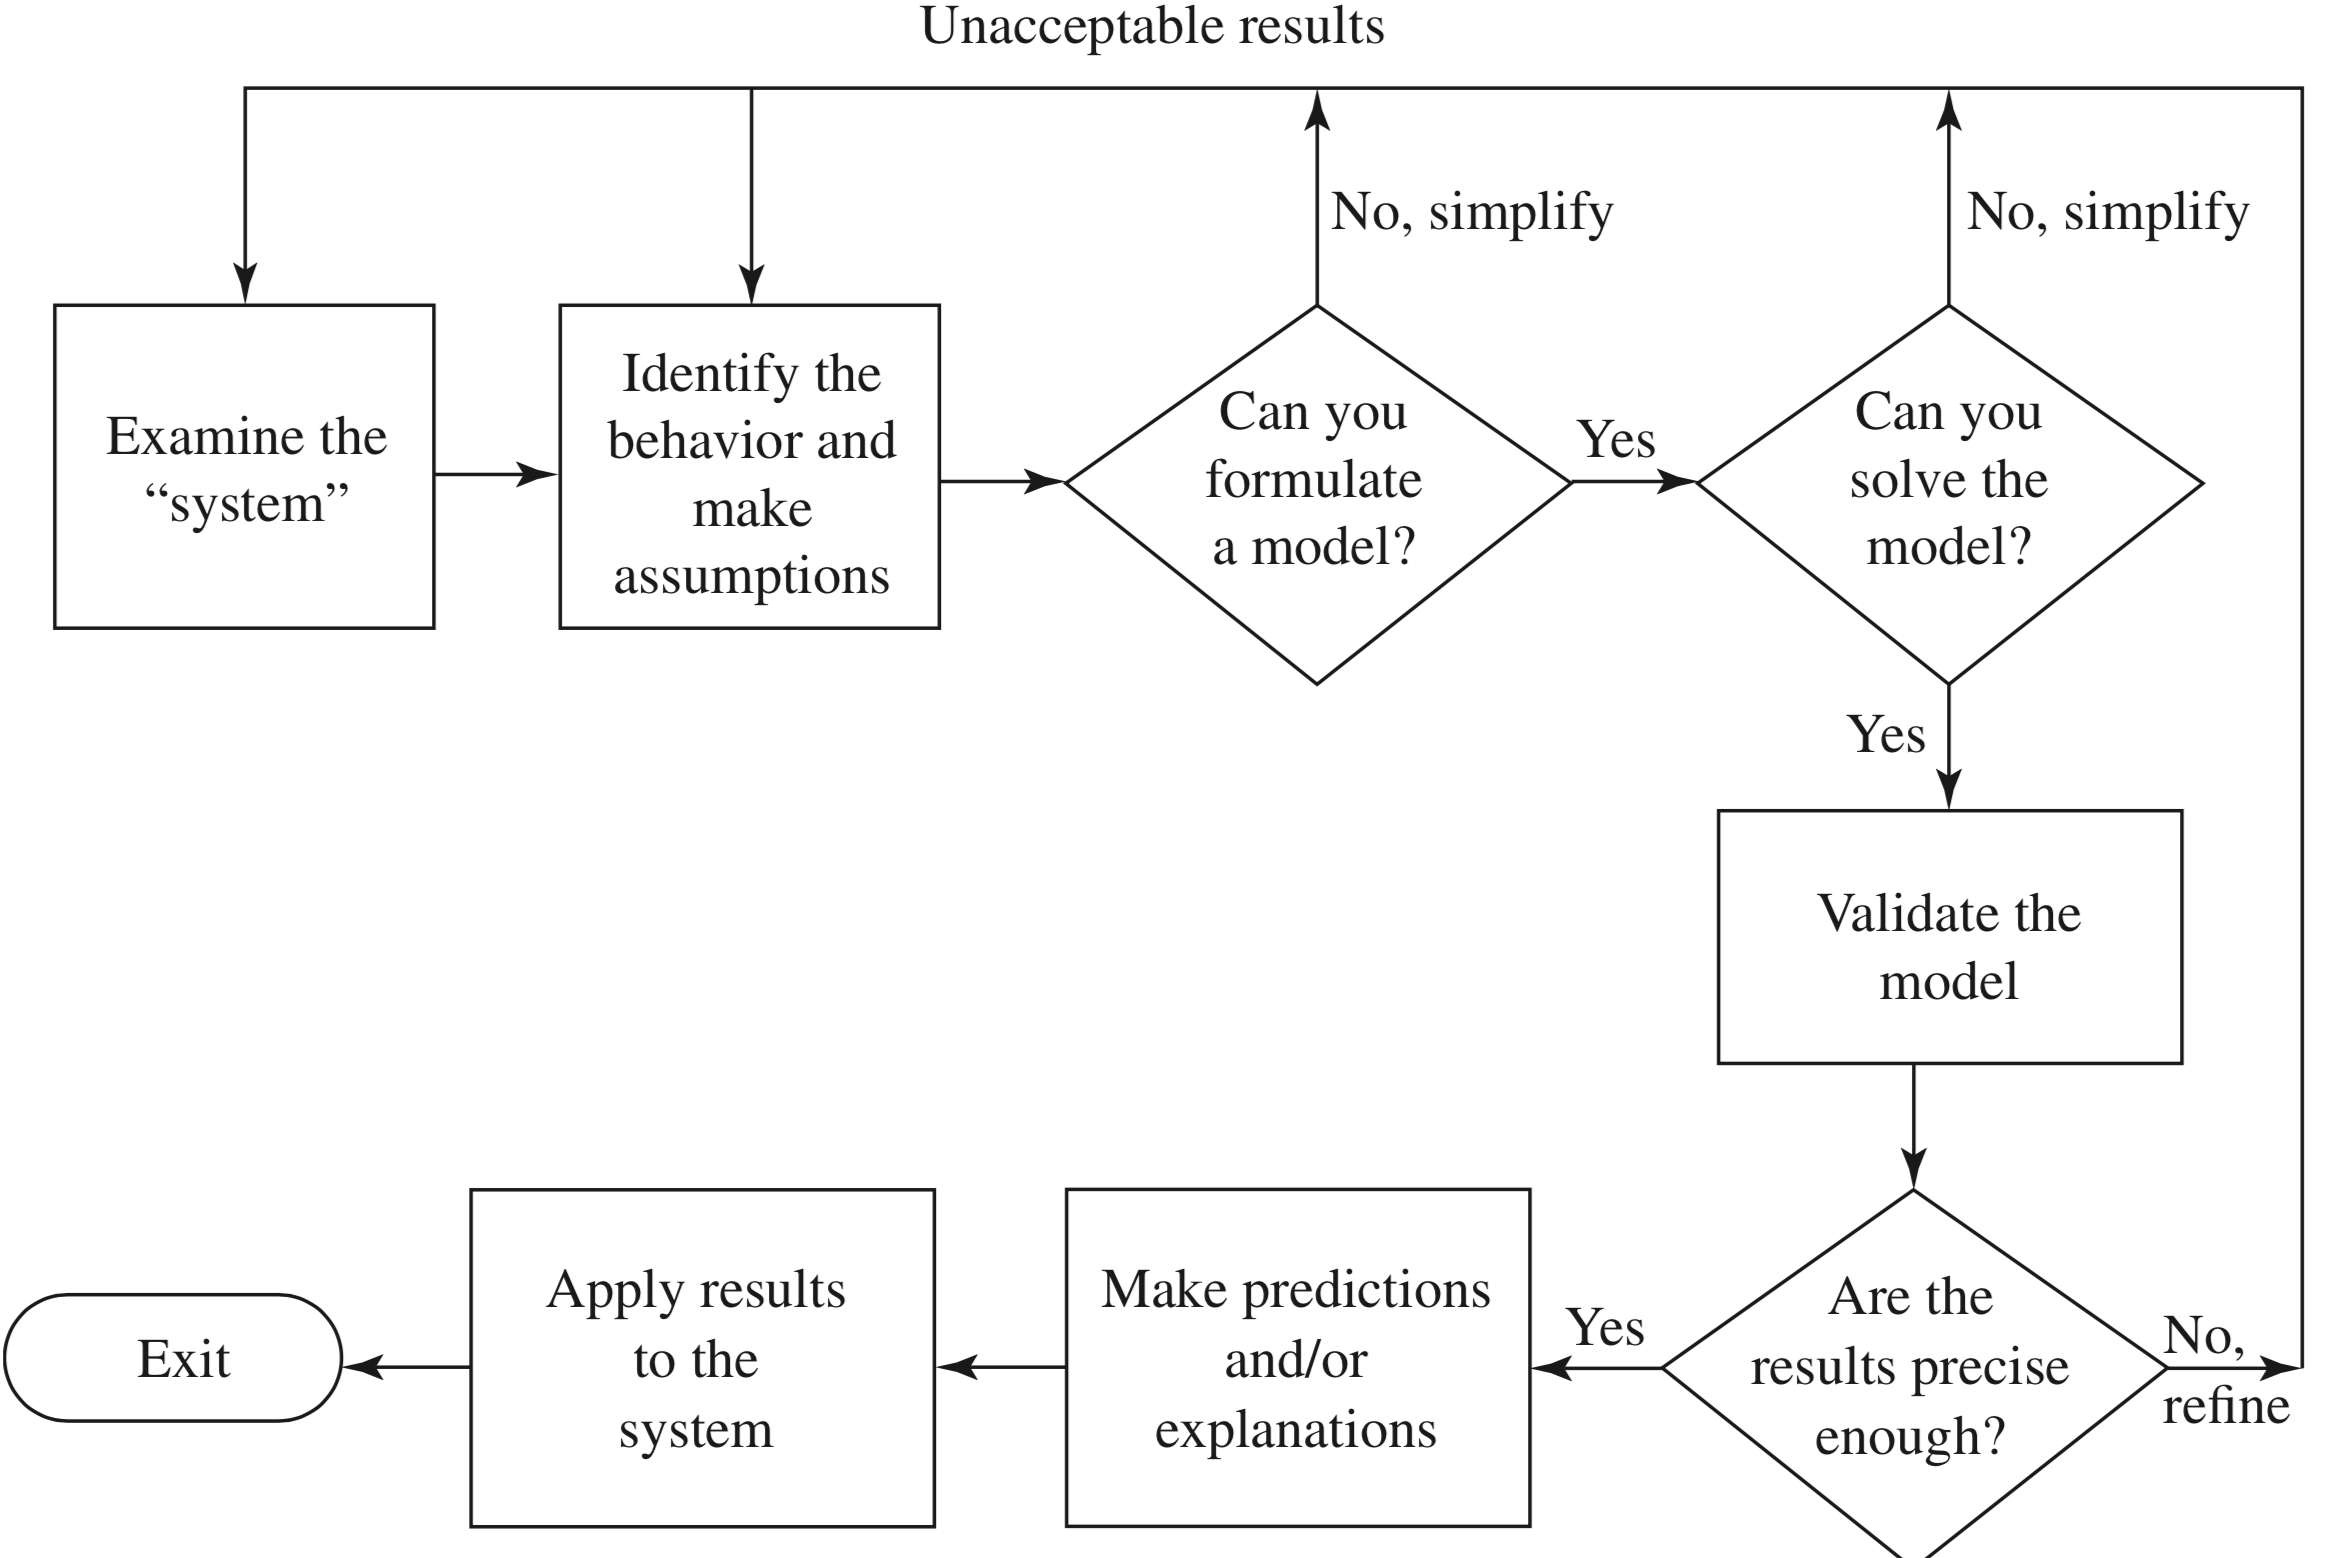
\includegraphics[width=.8\textwidth{}]{modeliterate.png}
  \end{center}
  
\end{frame}

\begin{frame}{数学建模的艺术:根据需要简化或改进模型}

  \begin{table}[ht]
    \centering
    \begin{tabular}{ll}
      模型简化 & 模型改进\\
      \hline{}
      1. 限制问题的识别 & 1. 扩展问题\\
      2. 忽略一些变量 & 2. 考虑额外的变量\\
      3. 若干变量合并的效果 & 3. 仔细考虑每个变量\\
      4. 令某些变量为常数 & 4. 允许变量变化\\
      5. 假设简单的(线性)关系 & 5. 考虑非线性关系\\
      6. 融入更多的假设 & 6. 减少假设的数量
    \end{tabular}
  \end{table}

  \begin{description}
  \item[强健] 结论并不依赖于精确地满足其假设
  \item[脆弱] 结论依赖于要满足某些类型的条件
  \item[敏感性] 模型结论所依赖的某个条件变化时结论的变化程度
  \end{description}

\end{frame}

\begin{frame}{利用比例性进行建模}
  \begin{block}{定义}
    $y \propto x$ 当且仅当对某个常数$k>0$,有$y=kx$
  \end{block}

  \begin{itemize}
  \item $y \propto x^2 \Rightarrow y=k_1x^2$
  \item $y \propto \ln x \Rightarrow y=k_2\ln x$
  \item $y \propto e^x \Rightarrow y=k_3 e^x$
  \item $y \propto x, x \propto z \Rightarrow y \propto z$
  \end{itemize}

  \begin{center}
    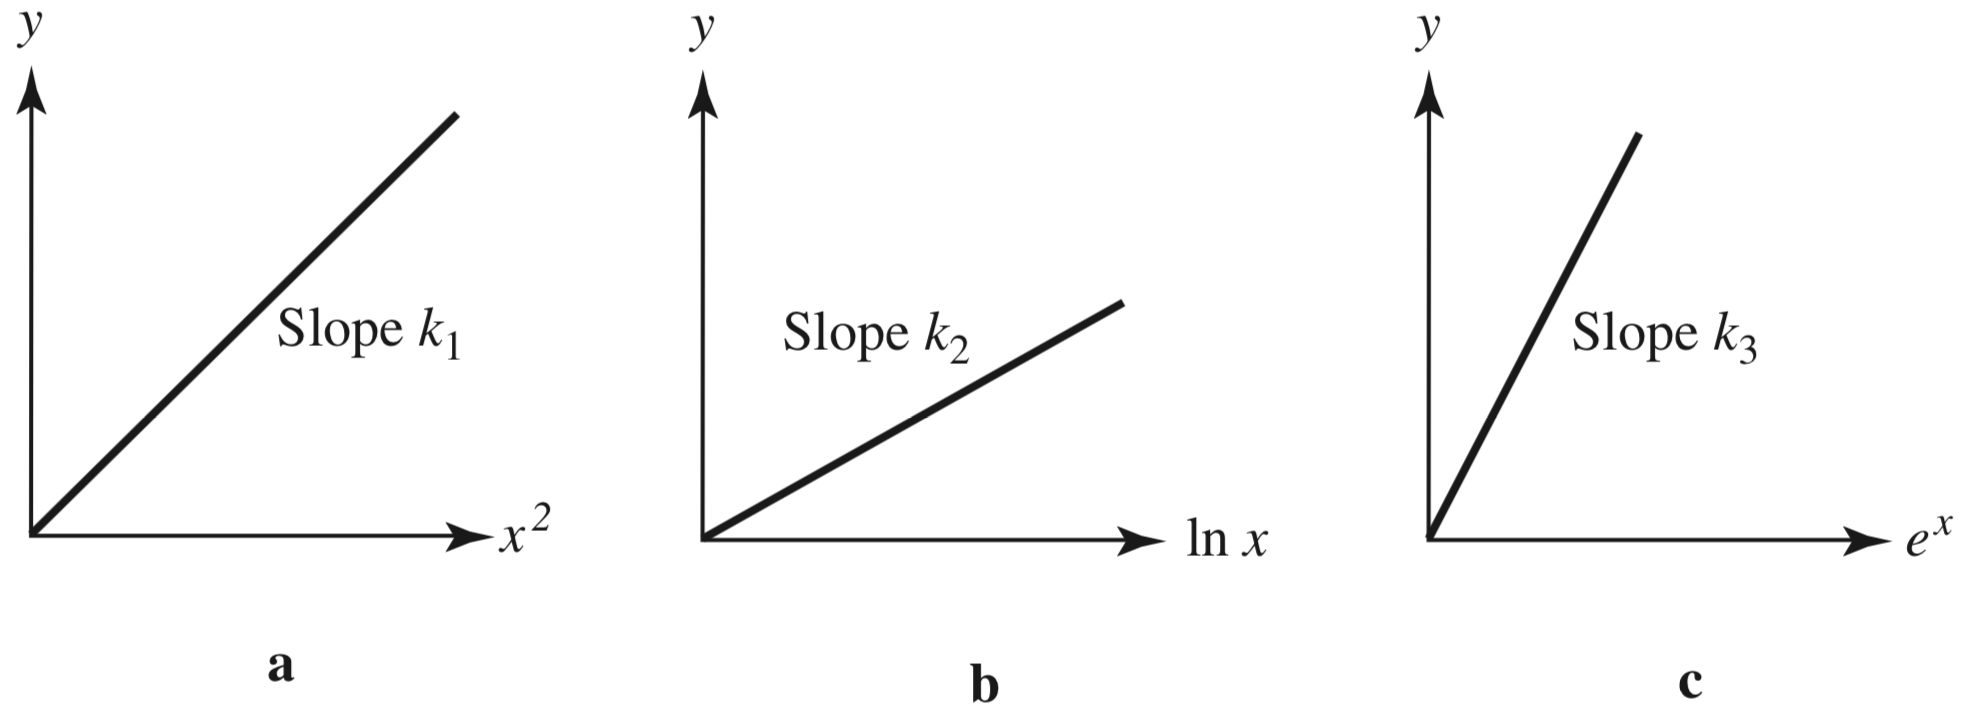
\includegraphics[width=.6\textwidth{}]{proptofig.png}
  \end{center}
\end{frame}

\begin{frame}{船的排水量}
  \begin{center}
    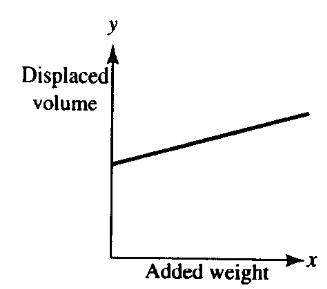
\includegraphics[width=.3\textwidth{}]{boatwater.png}
    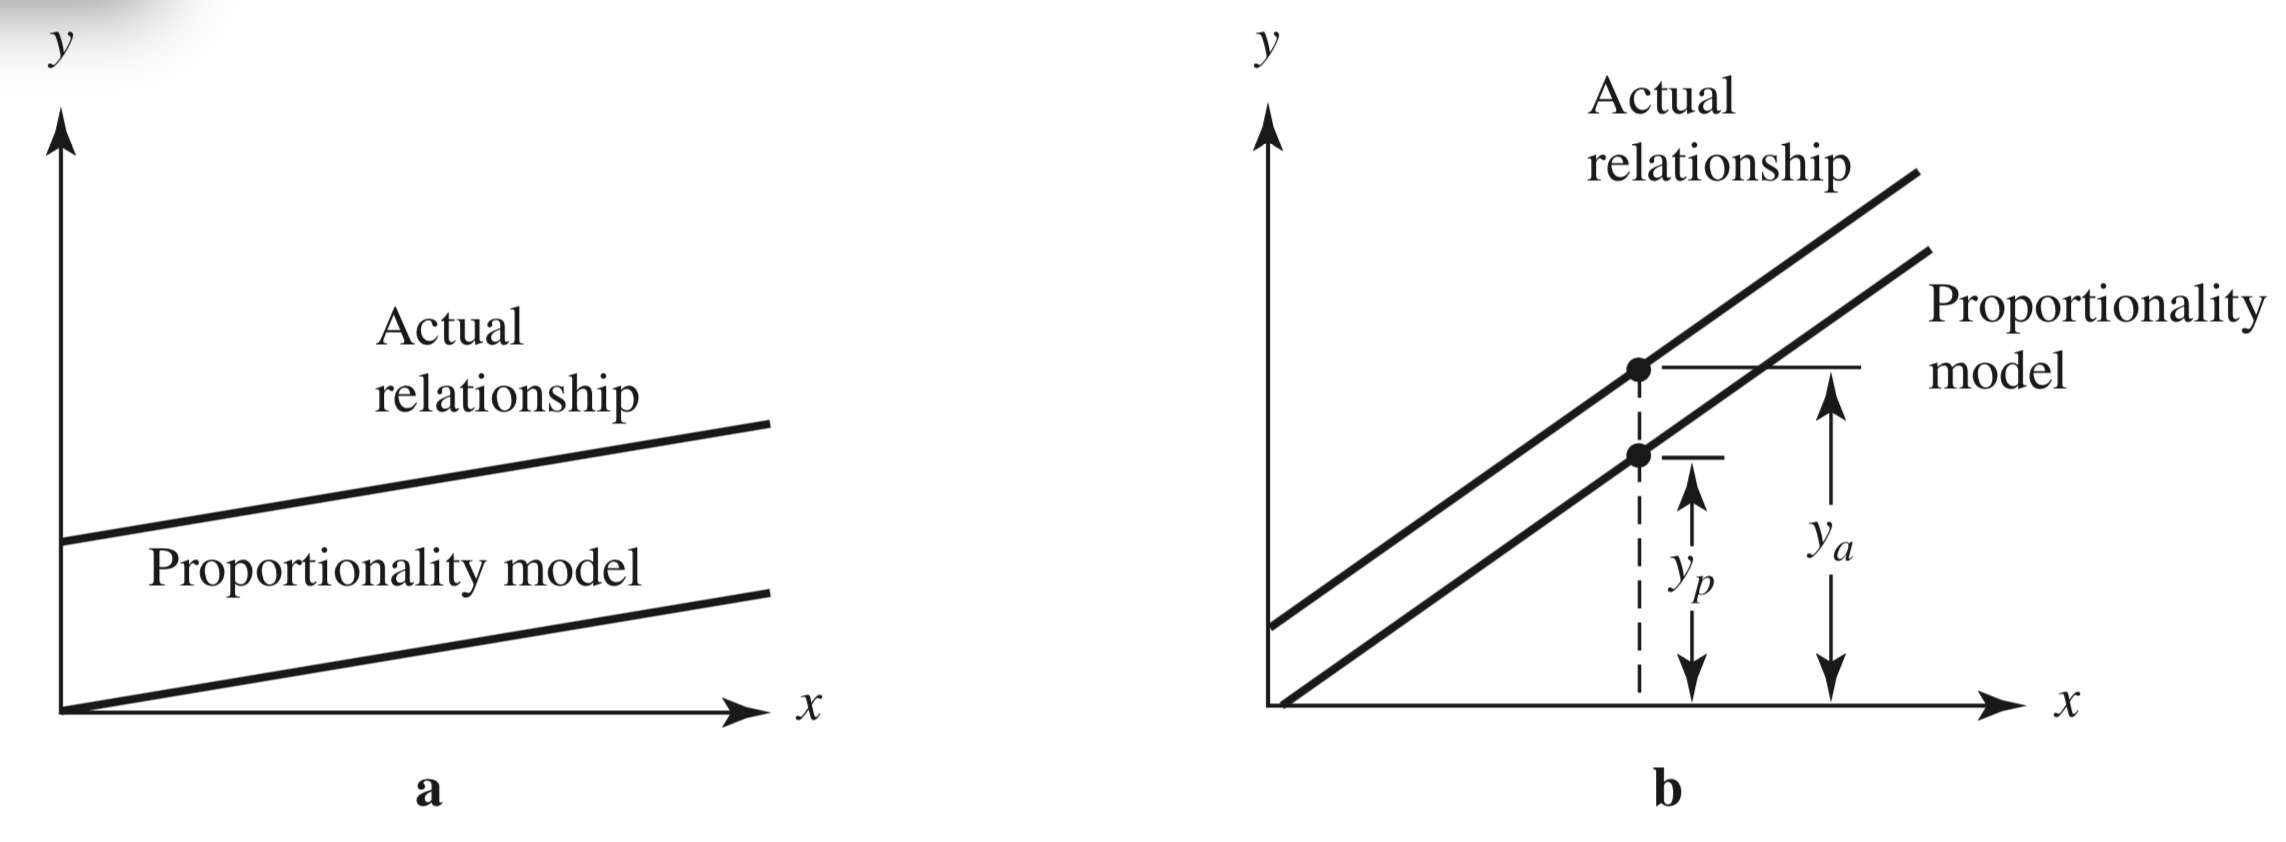
\includegraphics[width=.6\textwidth{}]{propapprox.png}
  \end{center}
\end{frame}

\begin{frame}{著名的比例性定律}
  \begin{center}
    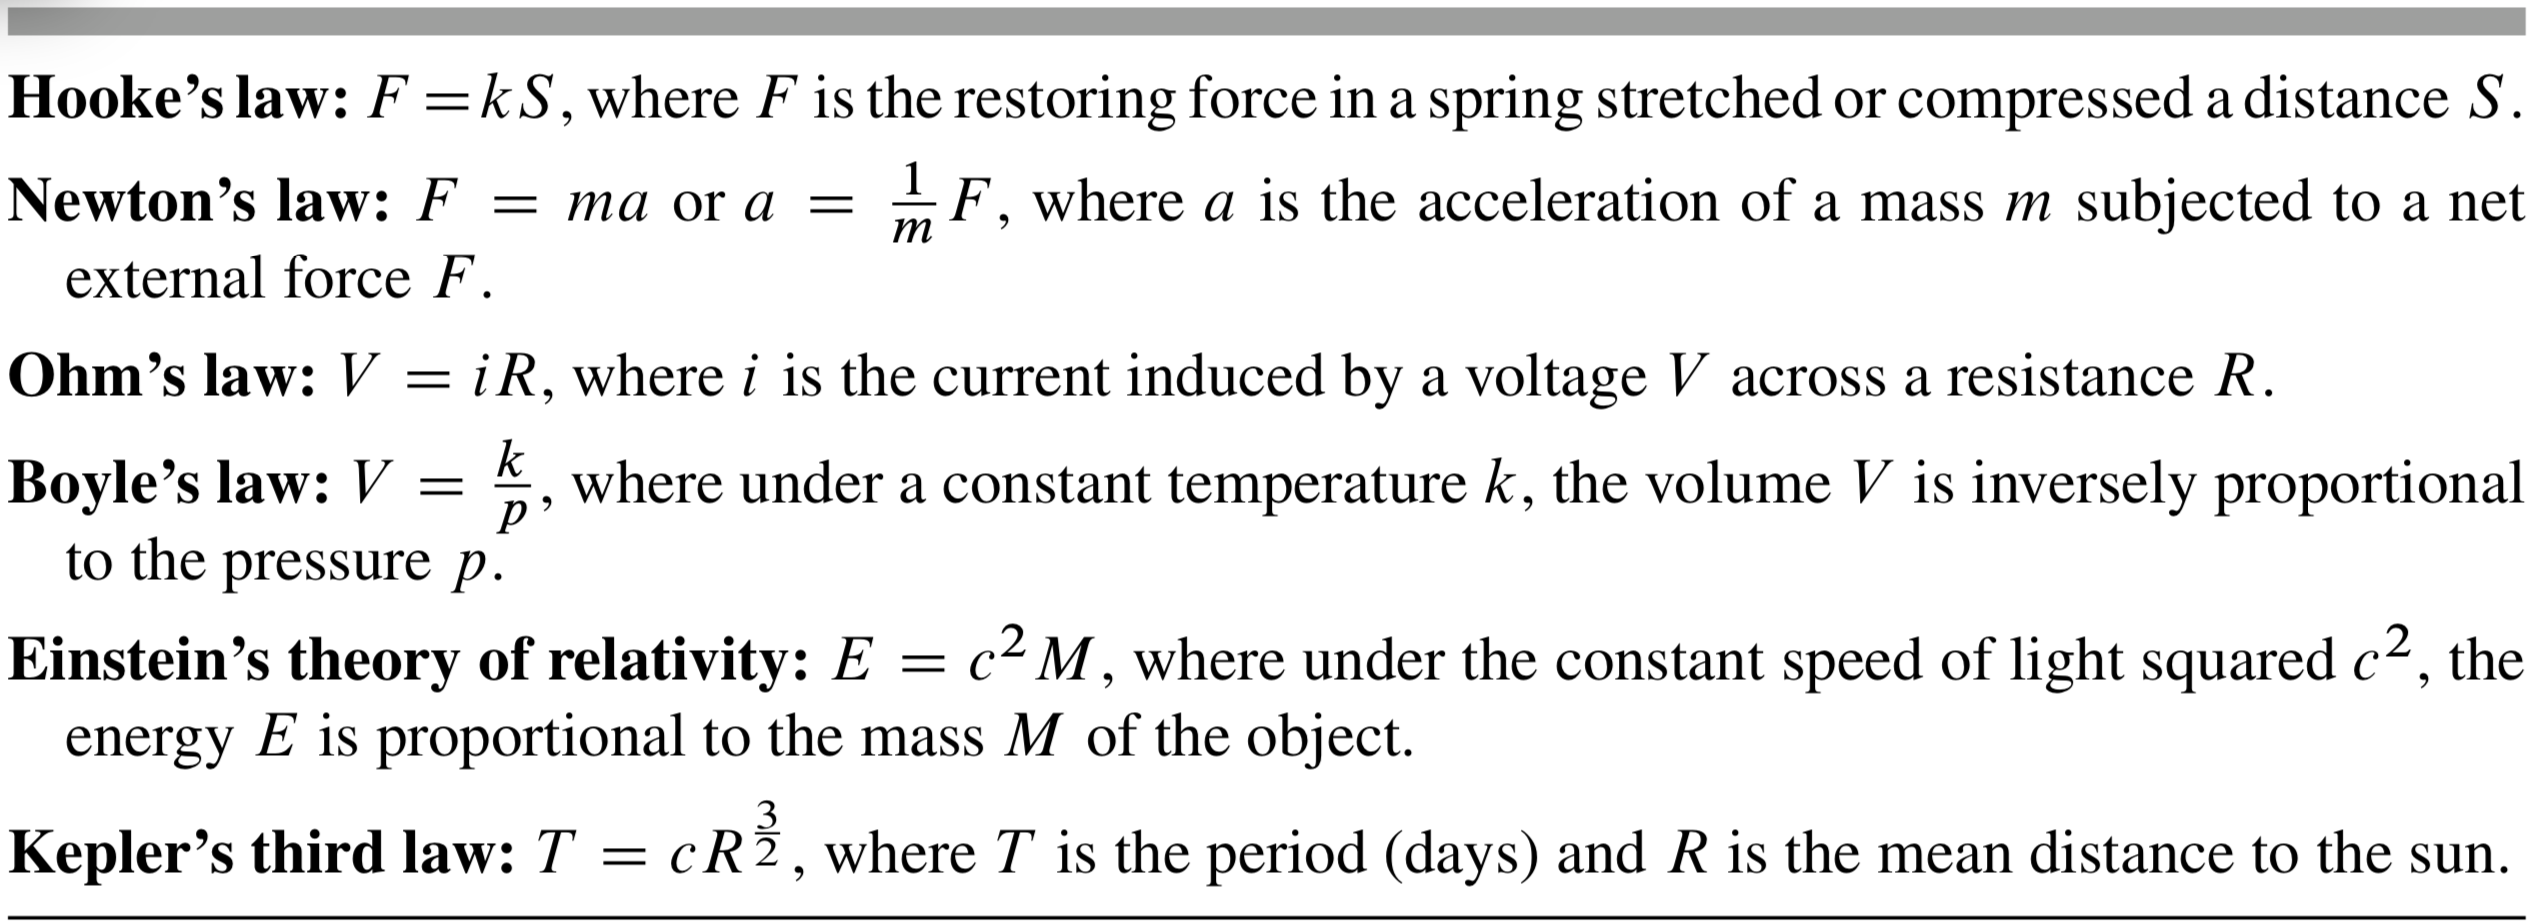
\includegraphics[width=.8\textwidth{}]{proptheory.png}
  \end{center}
\end{frame}

\begin{frame}{开普勒第三定律}
  $T=cR^{\frac{3}{2}}$, 其中$T$是周期(天数)而$R$是到太阳的平均距离

  \begin{center}
    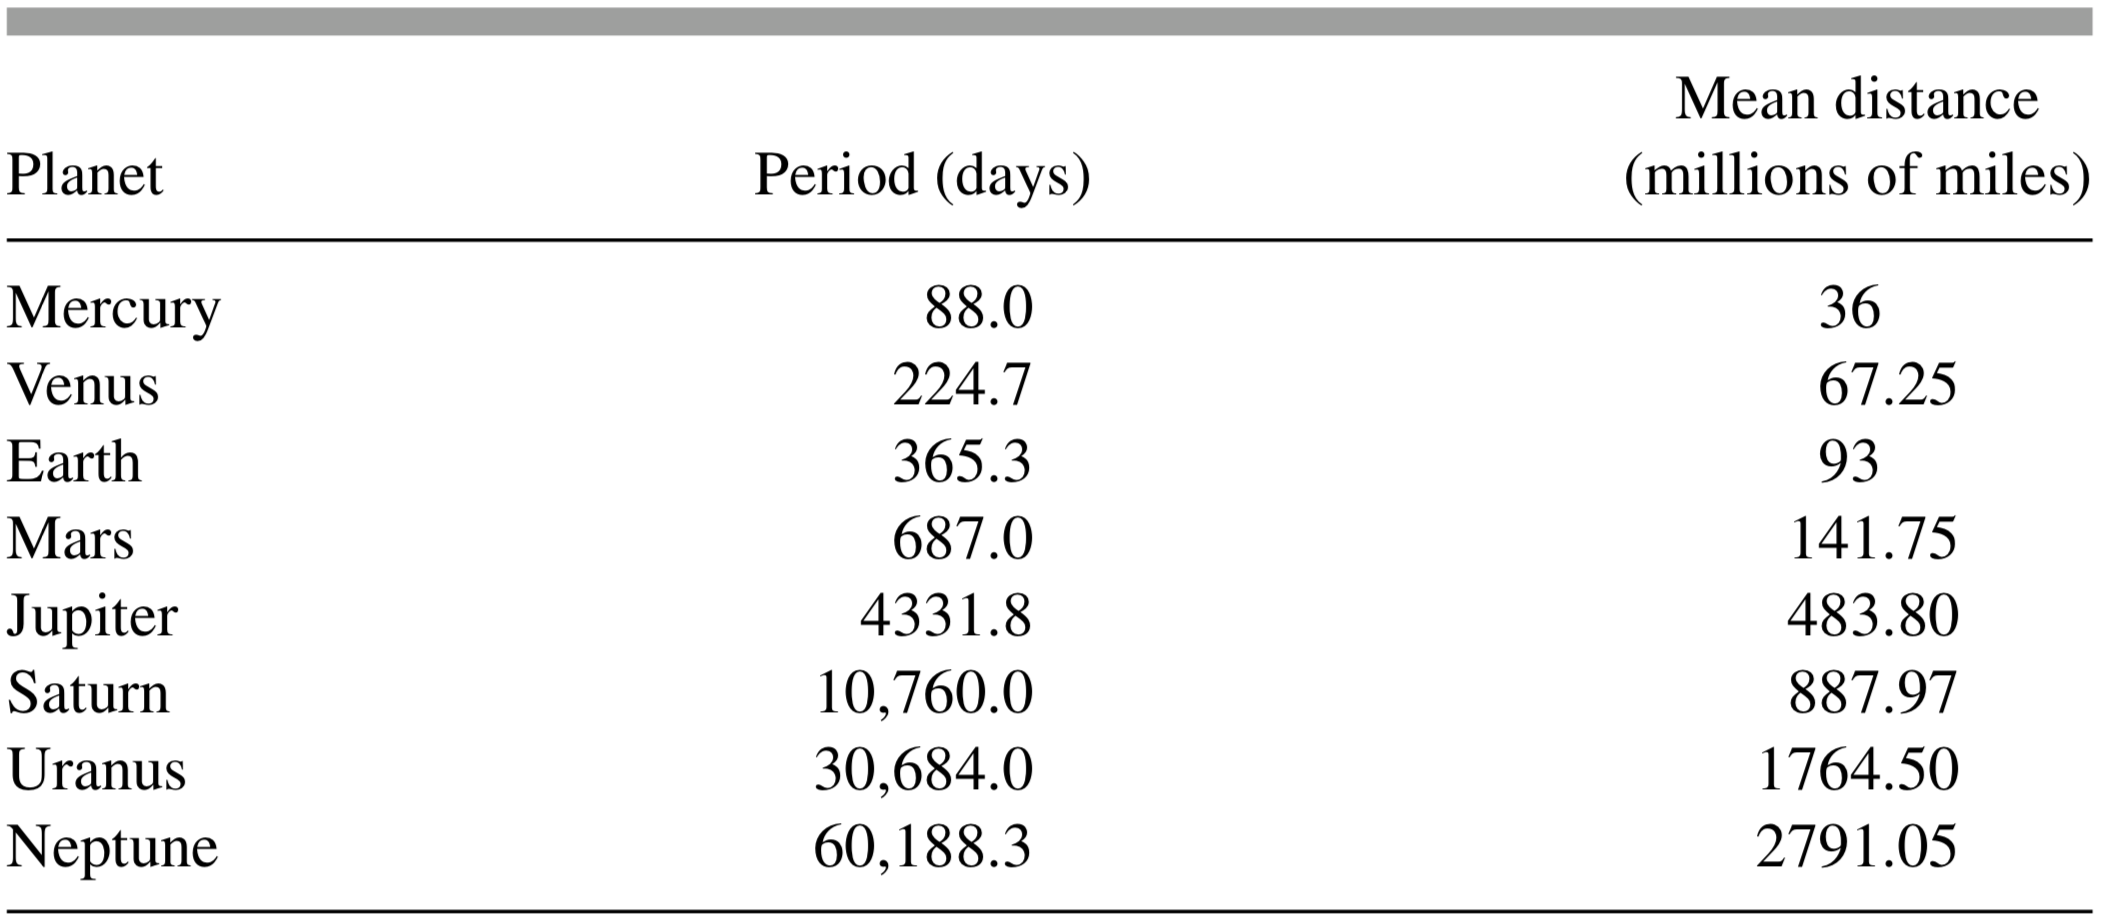
\includegraphics[width=.45\textwidth{}]{keplertable.png}
    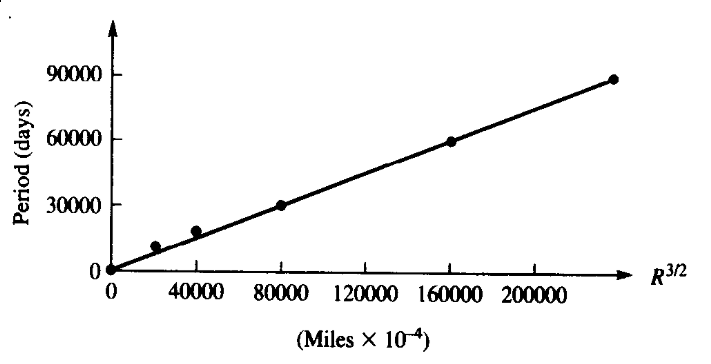
\includegraphics[width=.45\textwidth{}]{keplerfig.png}
  \end{center}

  \[
  c = \frac{90466.8-88}{220869.1-216} \approx 0.410
  \]
  
\end{frame}

\begin{frame}{对车辆停止距离建模}
  \begin{block}{一般规则}
    \begin{itemize}
    \item 每10英里的速度允许一辆车长度的跟随距离
    \item 看着前车刚驶过的点, 2秒之内到达表示太近了
    \end{itemize}
  \end{block}

  为使两条规则一致,在10英里/小时的情形:

  \begin{center}
    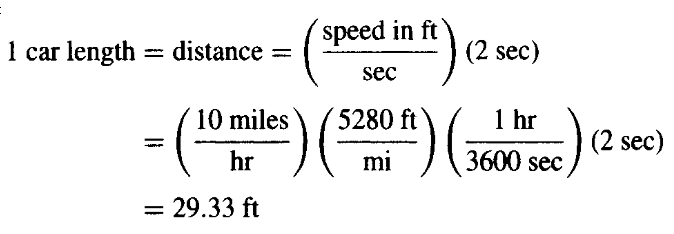
\includegraphics[width=.6\textwidth{}]{carformula.png}
  \end{center}

  如果车长只有15ft呢?

\end{frame}

\begin{frame}{观测数据}
  \begin{center}
    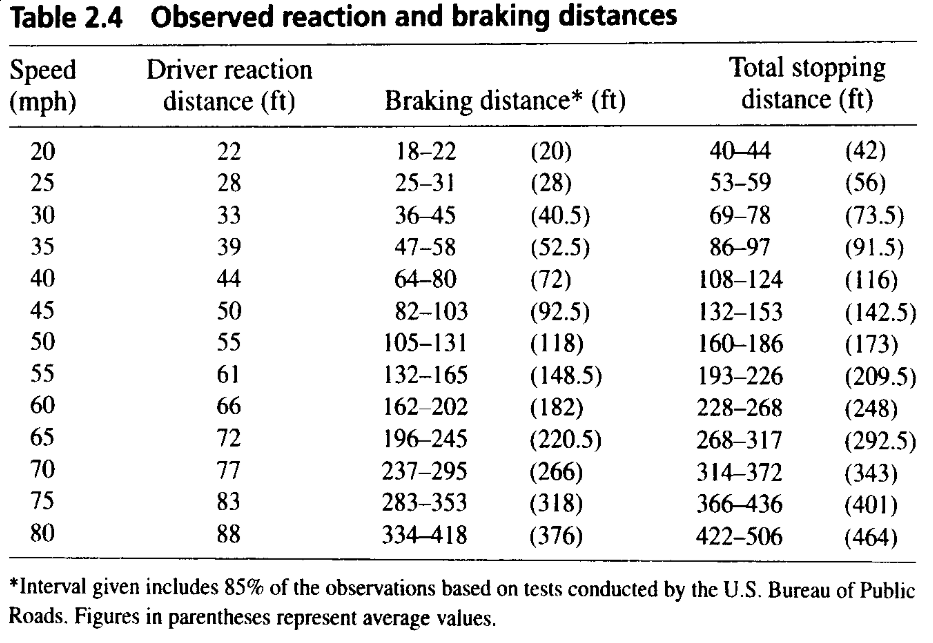
\includegraphics[width=.8\textwidth{}]{cardata.png}
  \end{center}
\end{frame}

\begin{frame}{反应距离}

  \begin{itemize}
  \item 总的停止距离 = 反应距离 + 刹车距离
  \item 反应距离 = $f$(反应时间, 速率)
  \item 假设反应时间内汽车以原速率运行: $d_r = t_rv$
  \item 验证:
  \end{itemize}

  \begin{center}
    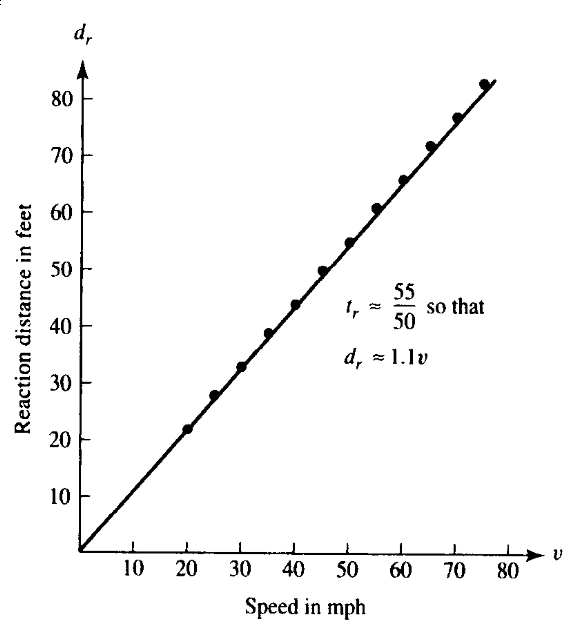
\includegraphics[width=.4\textwidth{}]{dr.png}
  \end{center}
\end{frame}

\begin{frame}{刹车距离}

  \begin{itemize}
  \item 刹车距离 = $h$(重量, 速率)
  \item 所做的功 = $Fd_b=\frac{1}{2}mv^2$
  \item 假设刹车的最大减速不变,由$F=ma$可知, $F \propto m$
  \item 由上面两点可知,$d_b \propto v^2$
  \end{itemize}

  \begin{center}
    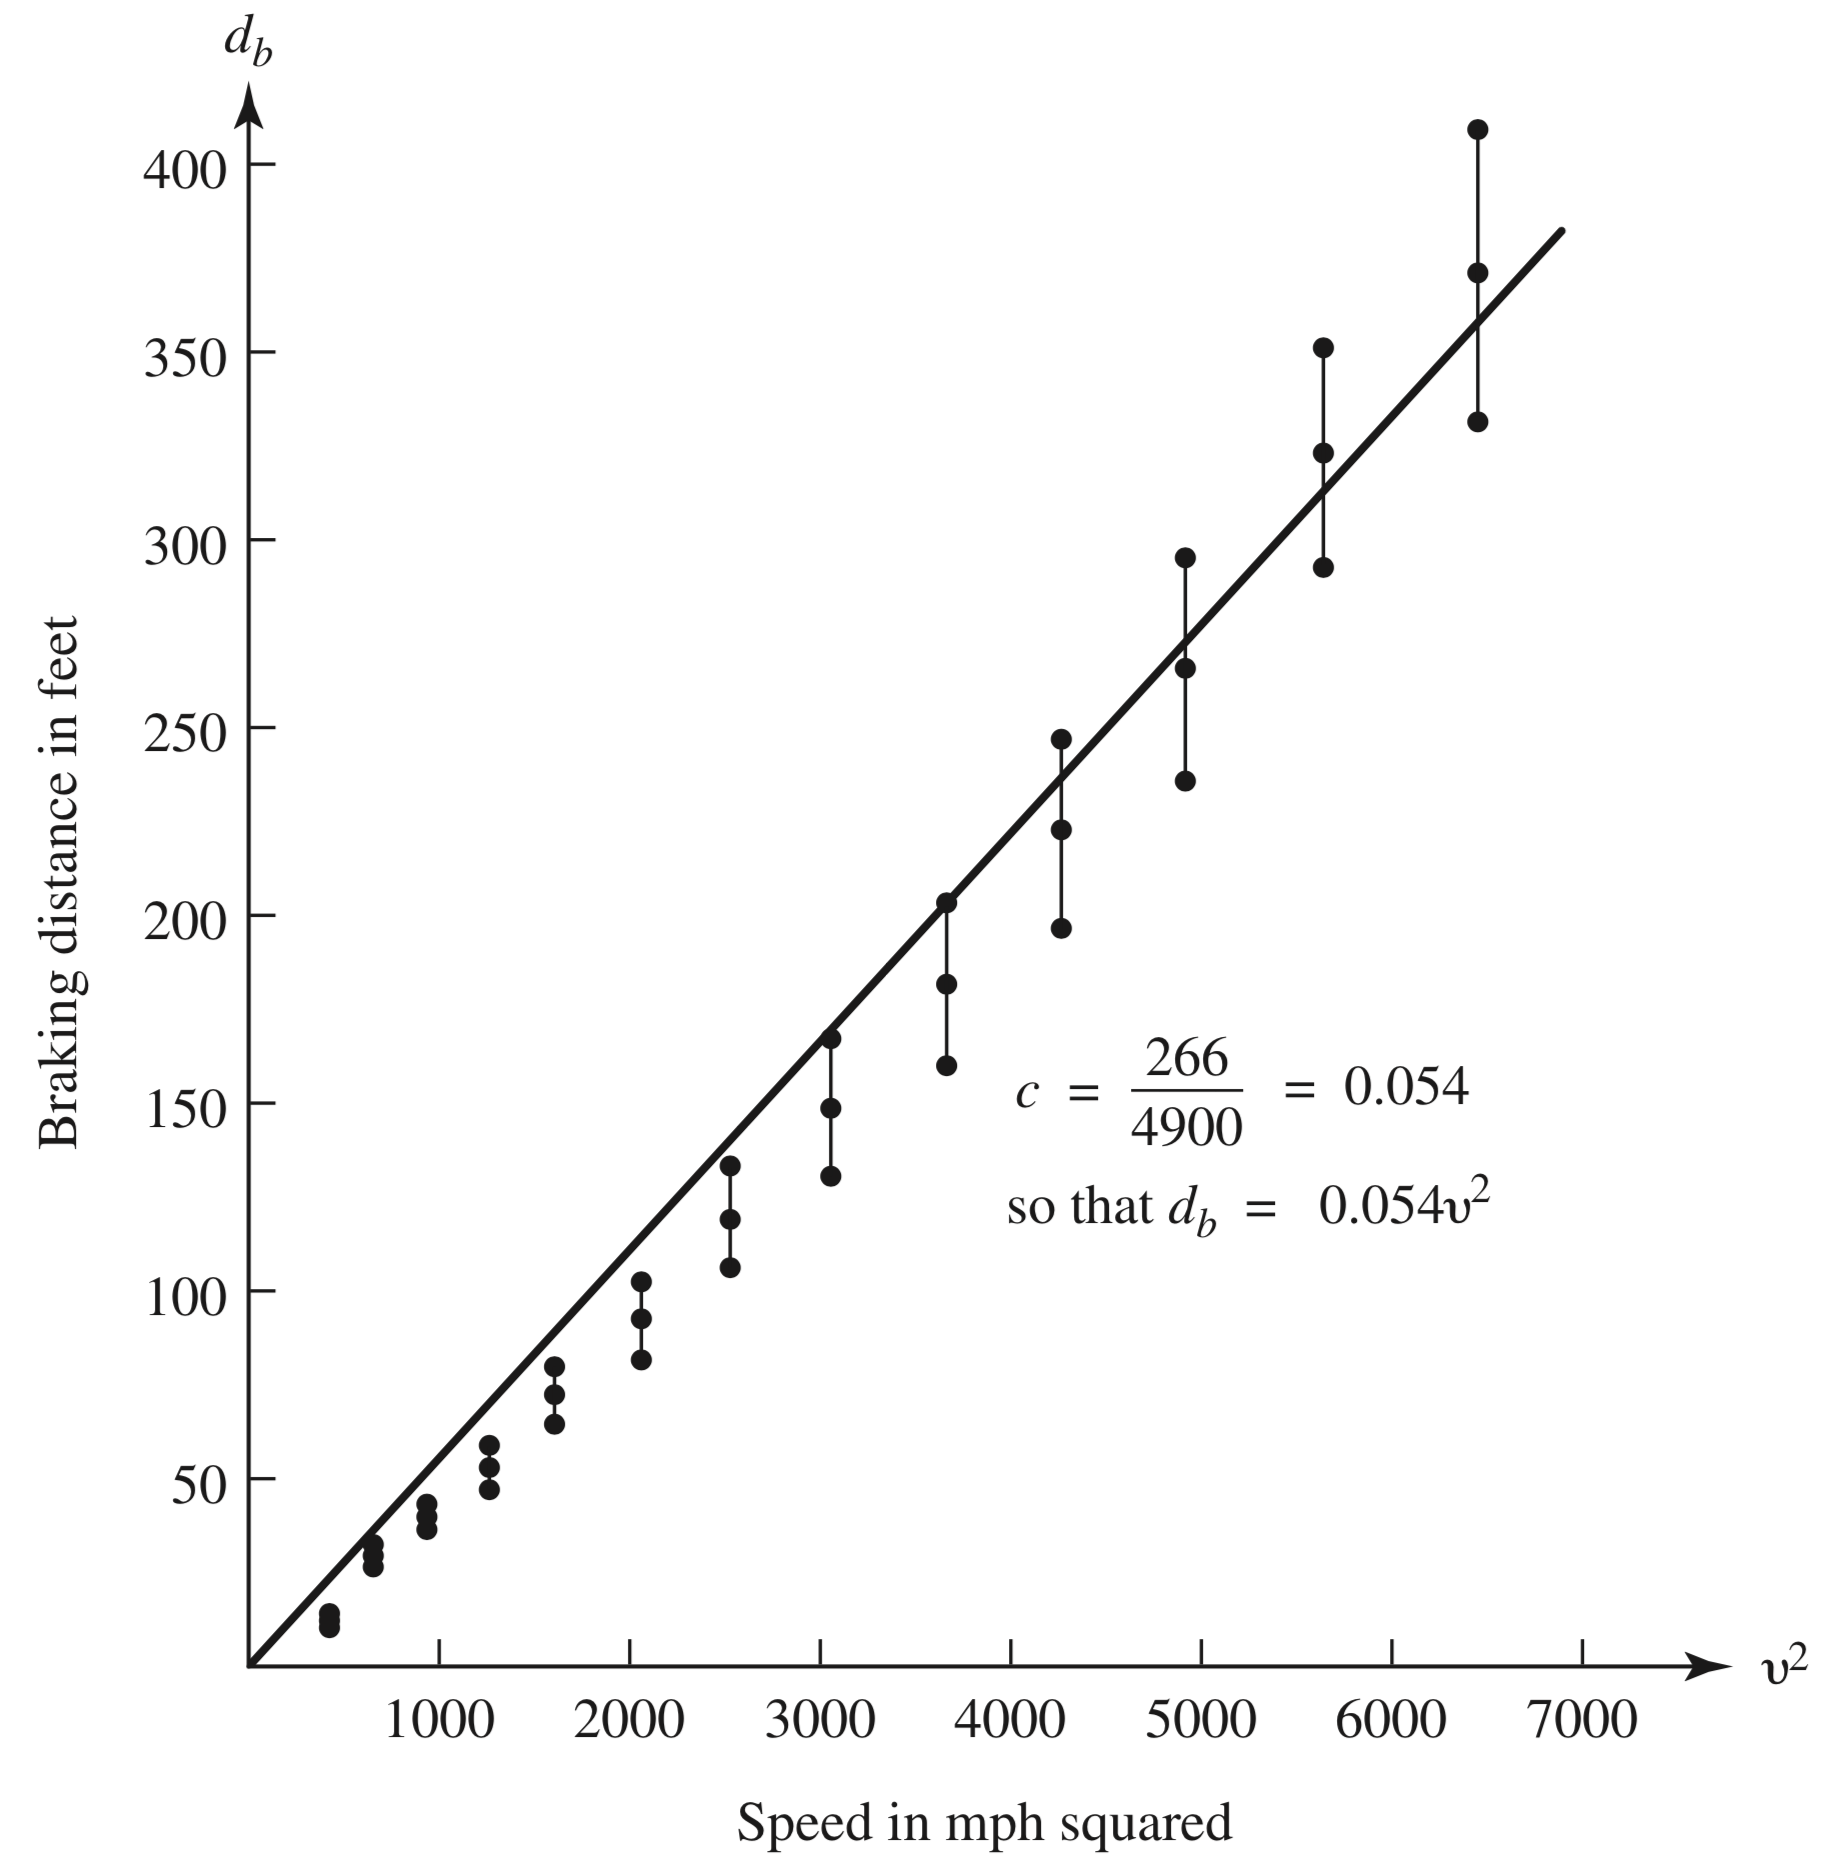
\includegraphics[width=.4\textwidth{}]{db.png}
  \end{center}
  
\end{frame}

\begin{frame}{模型验证}
  \[
  d = 1.1v + 0.054v^2
  \]

  \begin{center}
    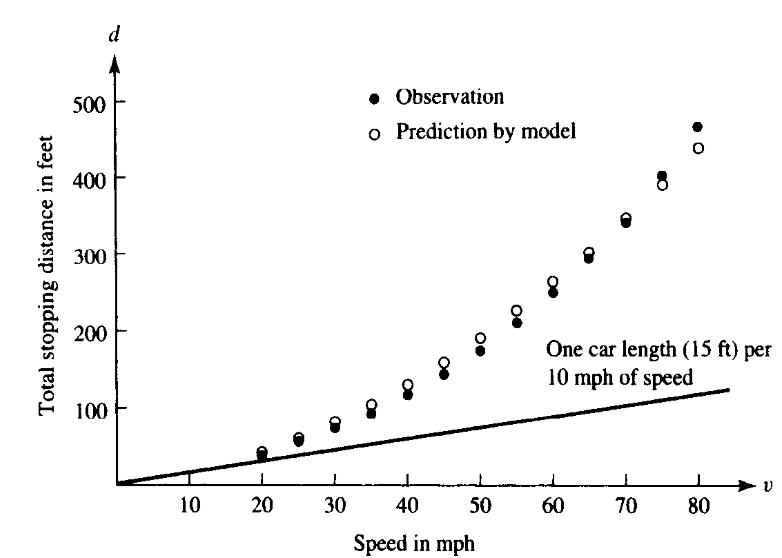
\includegraphics[width=.6\textwidth{}]{dcomp.png}
  \end{center}
\end{frame}

\begin{frame}{改进观察前车法则}

  \begin{center}
    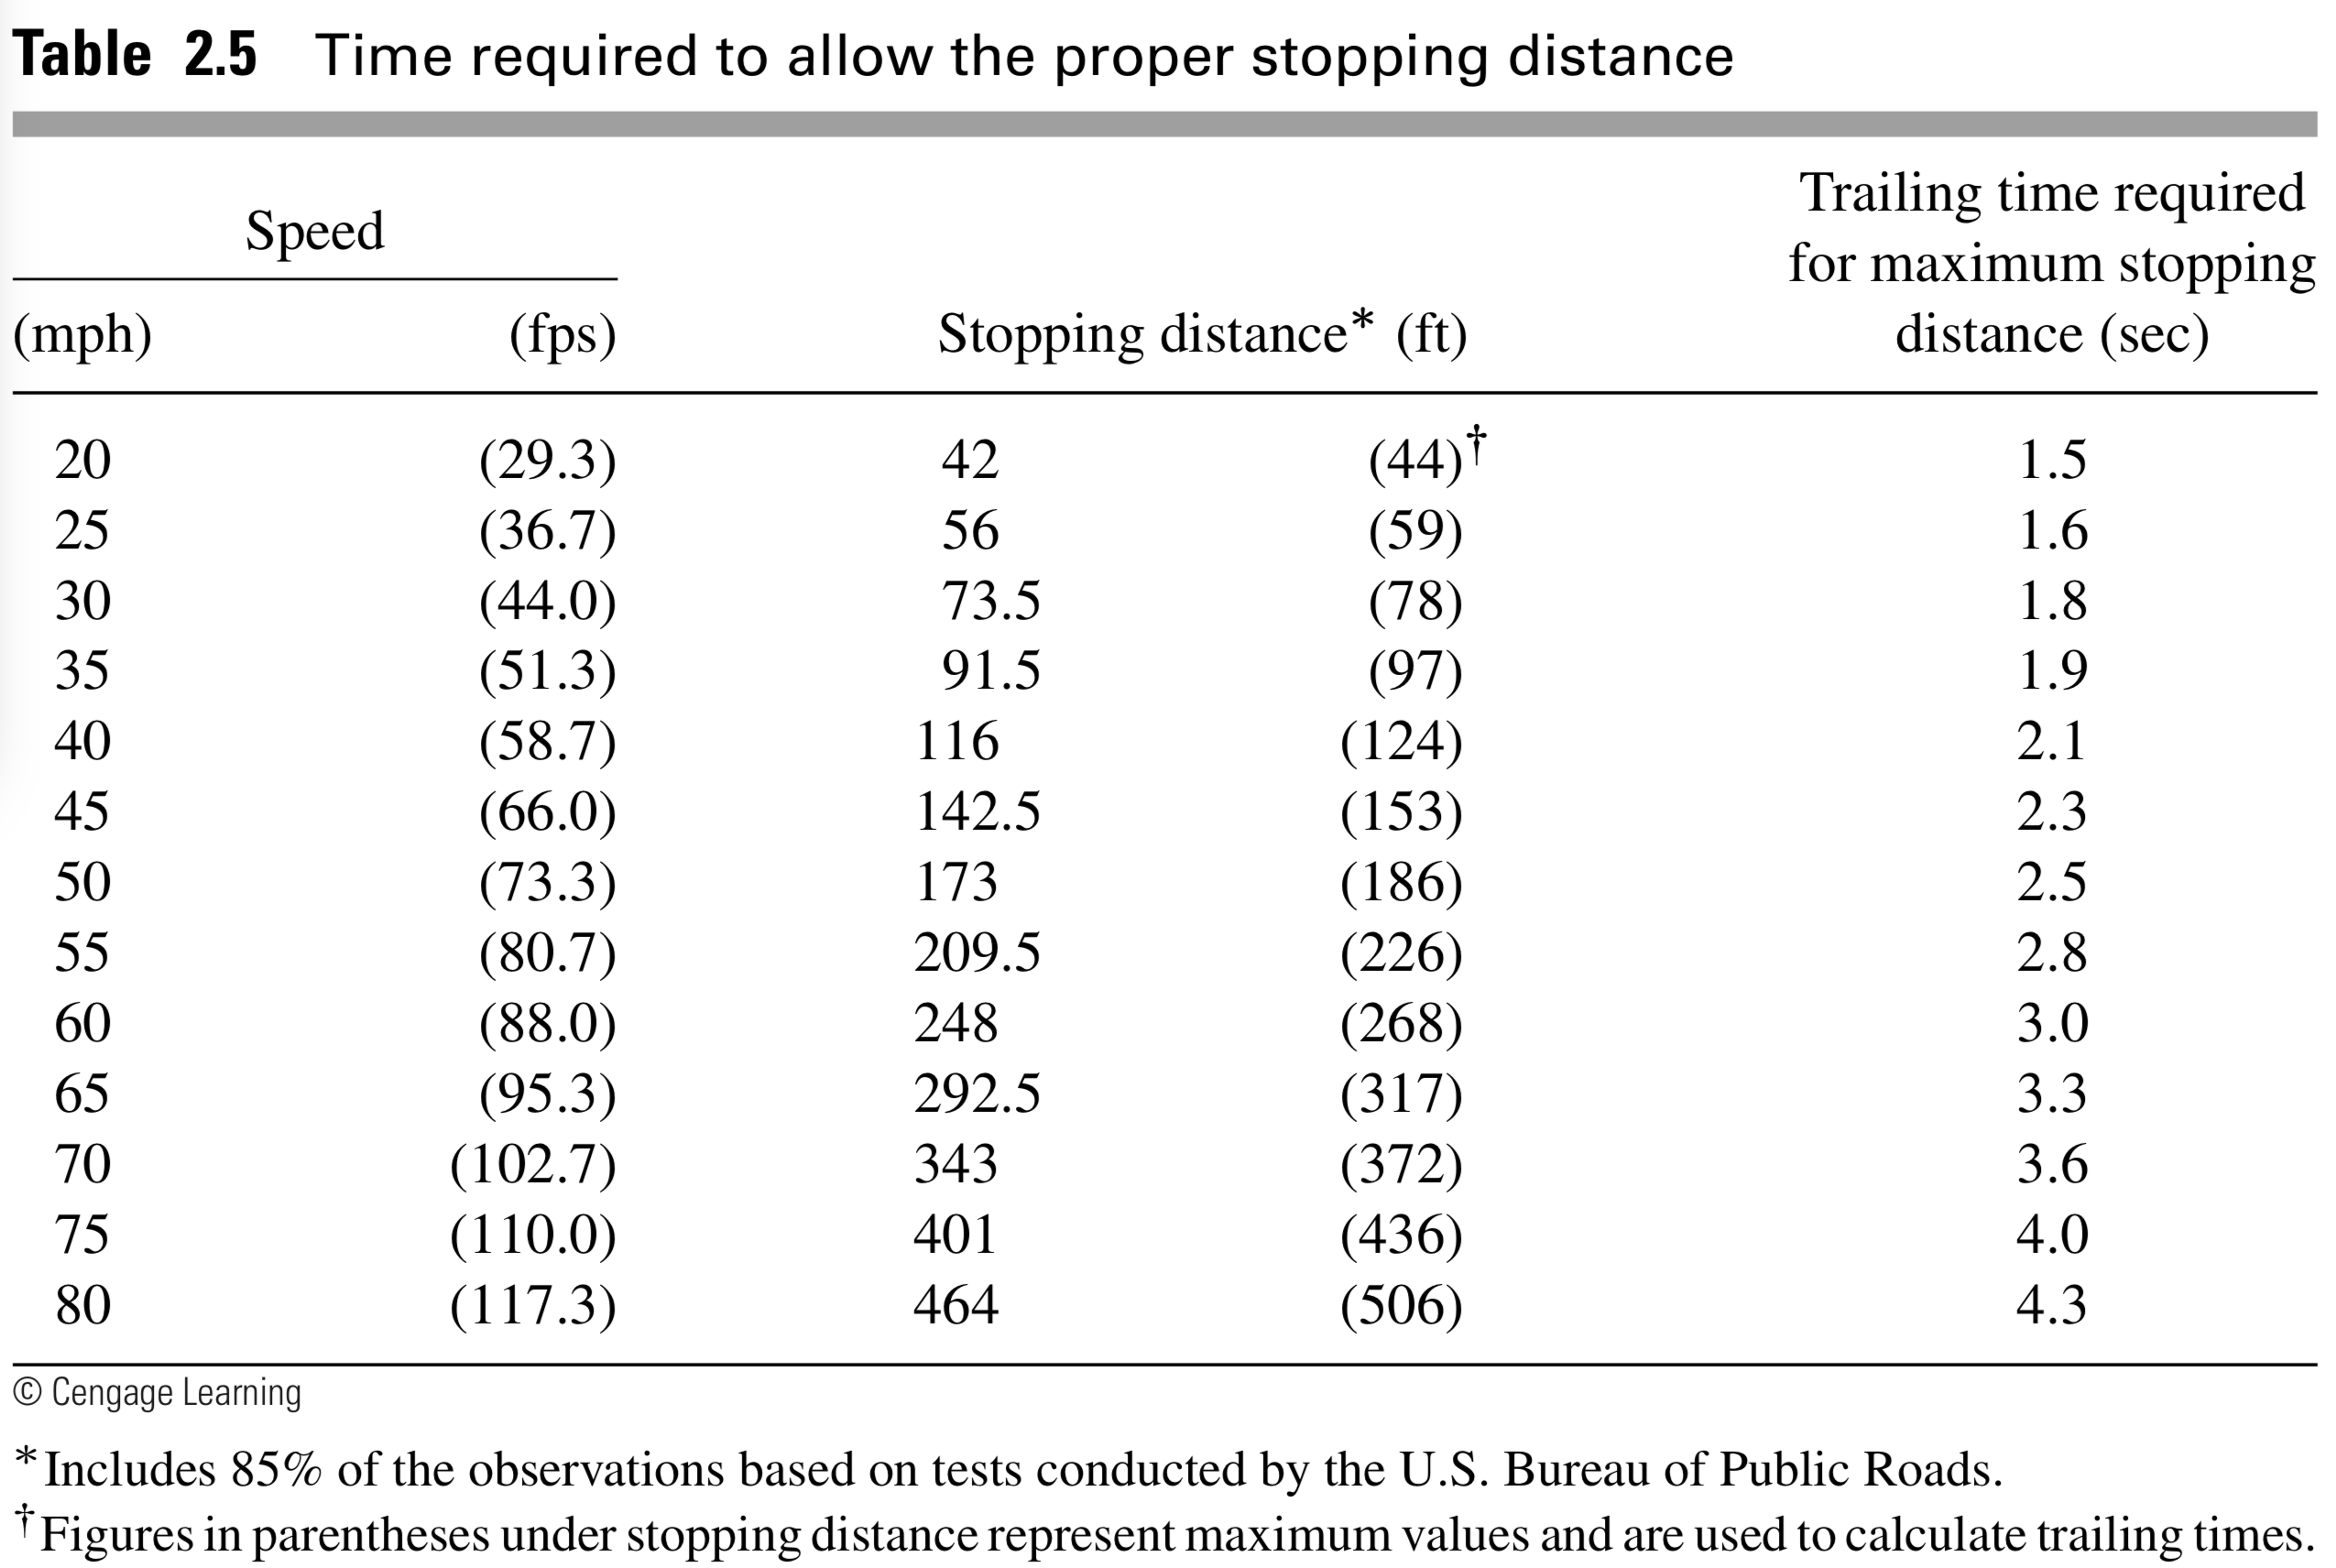
\includegraphics[width=.8\textwidth{}]{carobserve.png}
  \end{center}
  
\end{frame}

\begin{frame}{新法则}

  \begin{center}
    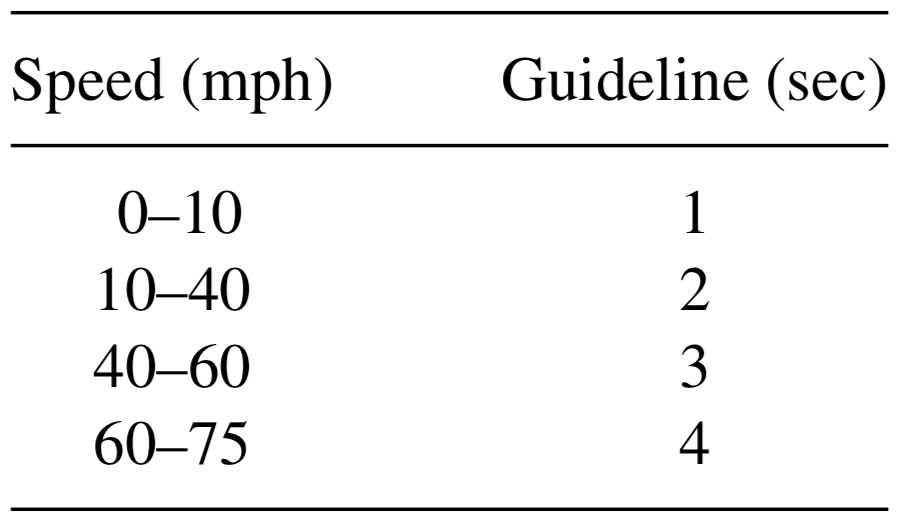
\includegraphics[width=.2\textwidth{}]{carnewlaw.png}
    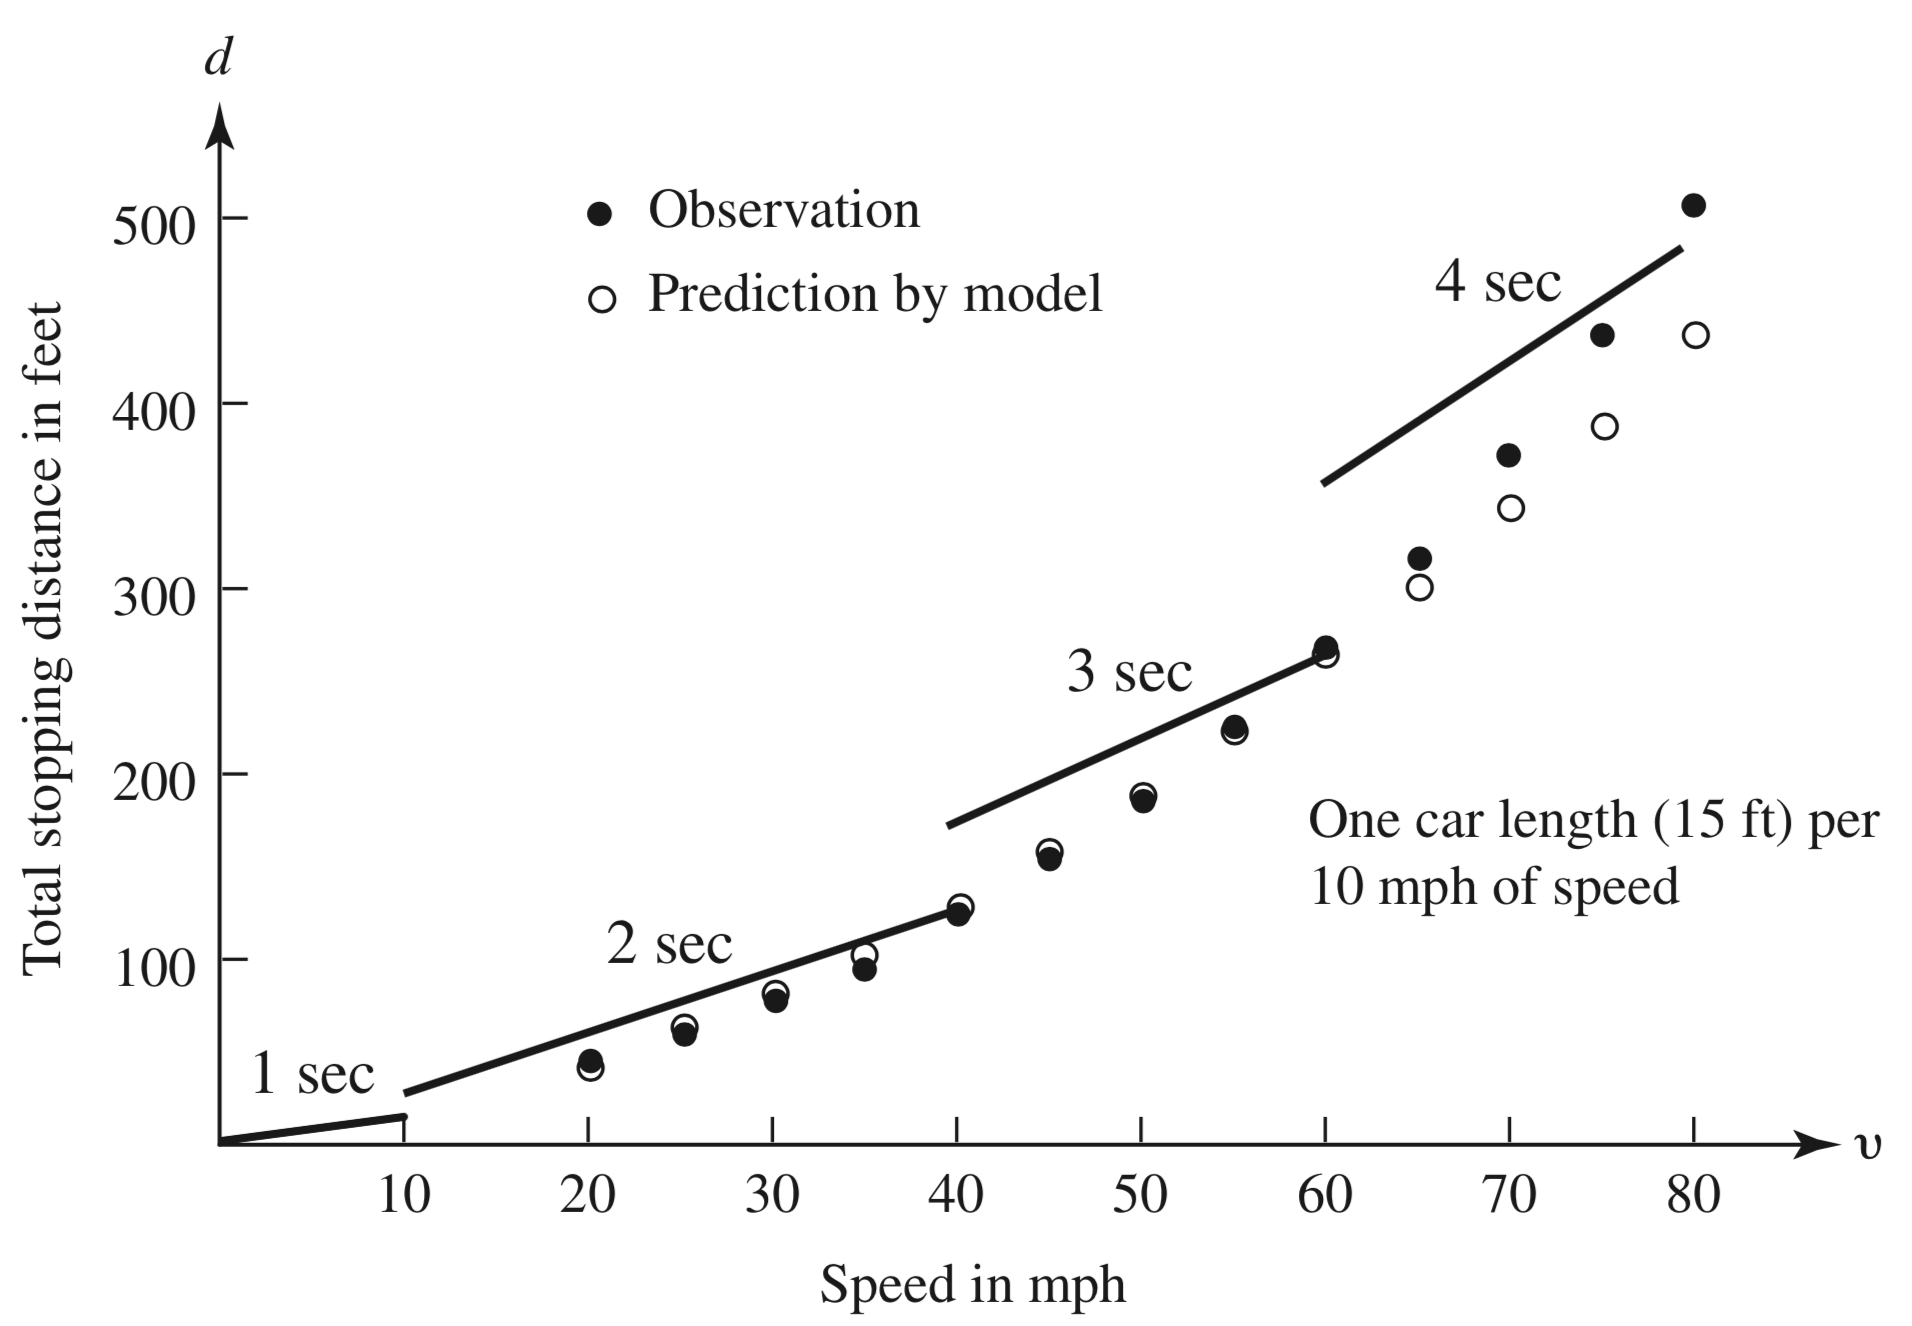
\includegraphics[width=.7\textwidth{}]{carfit.png}
  \end{center}
  
\end{frame}

\begin{frame}{利用几何相似性进行建模}
  \begin{center}
    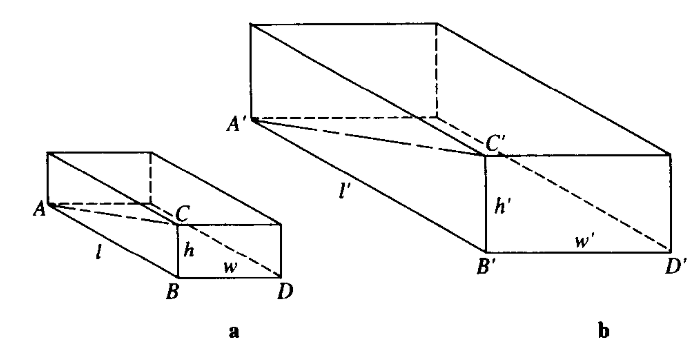
\includegraphics[width=.4\textwidth{}]{similar.png}
  \end{center}
  \begin{itemize}
  \item $\frac{l}{l'} = \frac{w}{w'} = \frac{h}{h'} = k$
  \item $\frac{V}{V'} = \frac{lwh}{l'w'h'} = k^3$
  \item $\frac{S}{S'} = \frac{2lh+2wh+2wl}{2l'h'+2w'h'+2w'l'} = k^2 = \frac{l^2}{l'^2}$
  \item $S \propto l^2, V \propto l^3$
  \item $y = f(l, S, V) = g(l, l^2, l^3)$
  \end{itemize}

\end{frame}

\begin{frame}{从不动的云层落下的雨滴}

  \begin{center}
    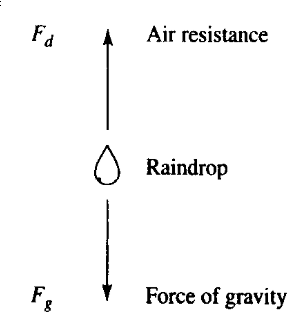
\includegraphics[width=.15\textwidth{}]{rain.png}
  \end{center}

  \begin{itemize}
  \item $F = F_g - F_d = ma$
  \item 终极速度时,加速度为0, 故$F_g - F_d = 0$或$F_g = F_d$
  \item 假设$F_d \propto Sv^2$
  \item $F_g \propto w, w \propto m \Rightarrow F_g \propto m$
  \item 假设雨滴几何相似: $S \propto l^2, V \propto l^3 \Rightarrow S \propto V^{2/3}$
  \item 质量和体积成正比$m \propto V$, 故$S \propto m^(2/3)$
  \item 因为$F_g = F_d$故$m \propto m^(2/3)v^2 \Rightarrow m^{1/6} \propto v$
  \item 雨滴的终极速度与其质量的六分之一次方成正比
  \end{itemize}
\end{frame}

\begin{frame}{钓鱼比赛建模}
  \begin{center}
    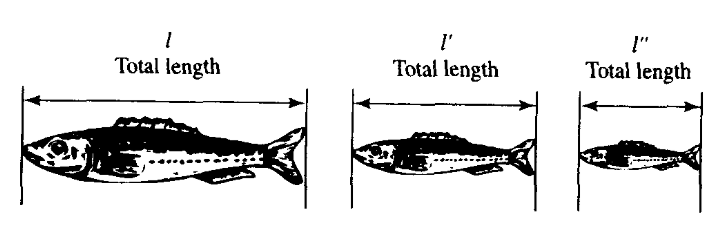
\includegraphics[width=.8\textwidth{}]{fish.png}
  \end{center}

  \begin{itemize}
  \item $V \propto l^3 \Rightarrow W \propto l^3$
  \end{itemize}
\end{frame}

\begin{frame}{验证模型}
  \begin{center}
    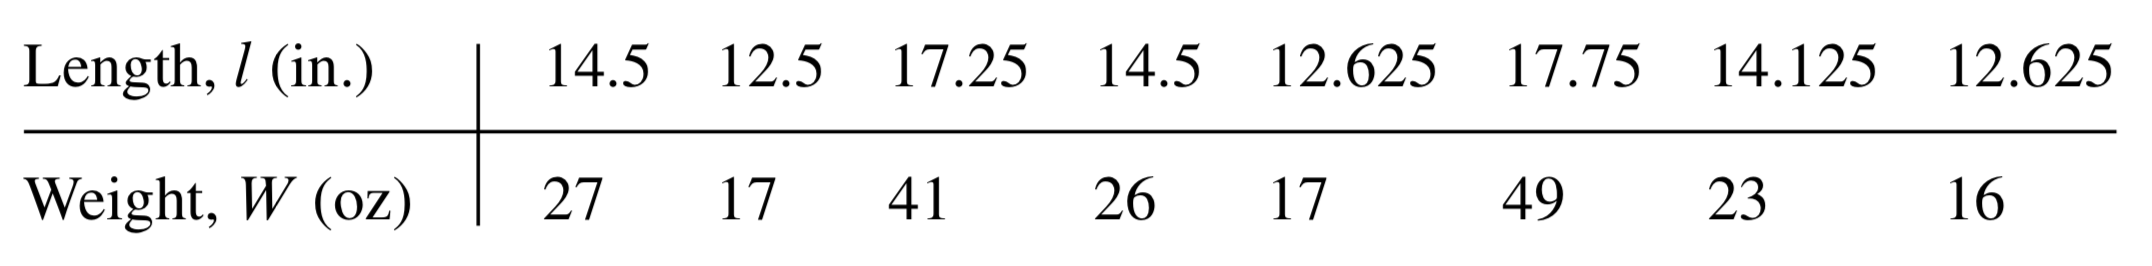
\includegraphics[width=.8\textwidth{}]{fishtab.png}
  \end{center}

  \begin{center}
    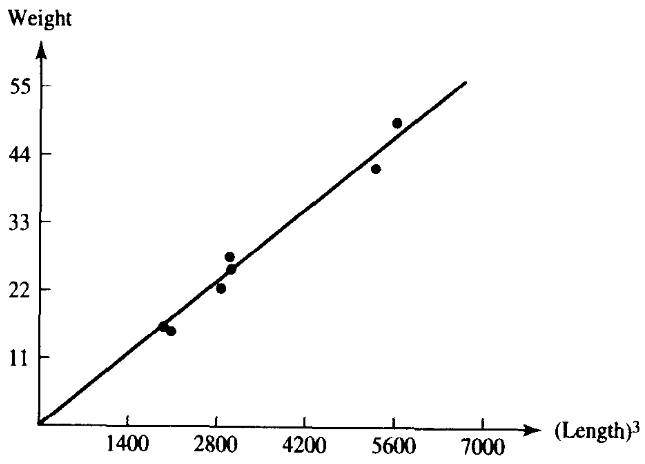
\includegraphics[width=.4\textwidth{}]{fishlen1.png}
    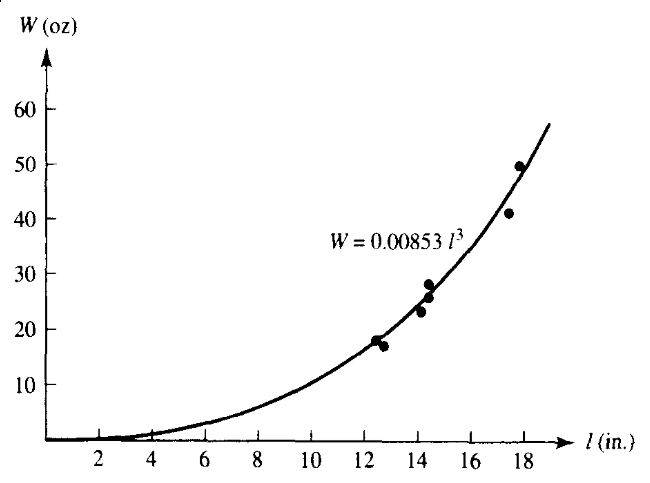
\includegraphics[width=.4\textwidth{}]{fishlen2.png}
  \end{center}
  \[
  W = 0.00853l^3
  \]
\end{frame}

\begin{frame}{改进模型}
  \begin{itemize}
  \item $V \approx l_{eff}A_{avg}$
  \item $V \propto lg^2 \Rightarrow W = klg^2$
  \end{itemize}
  \begin{center}
    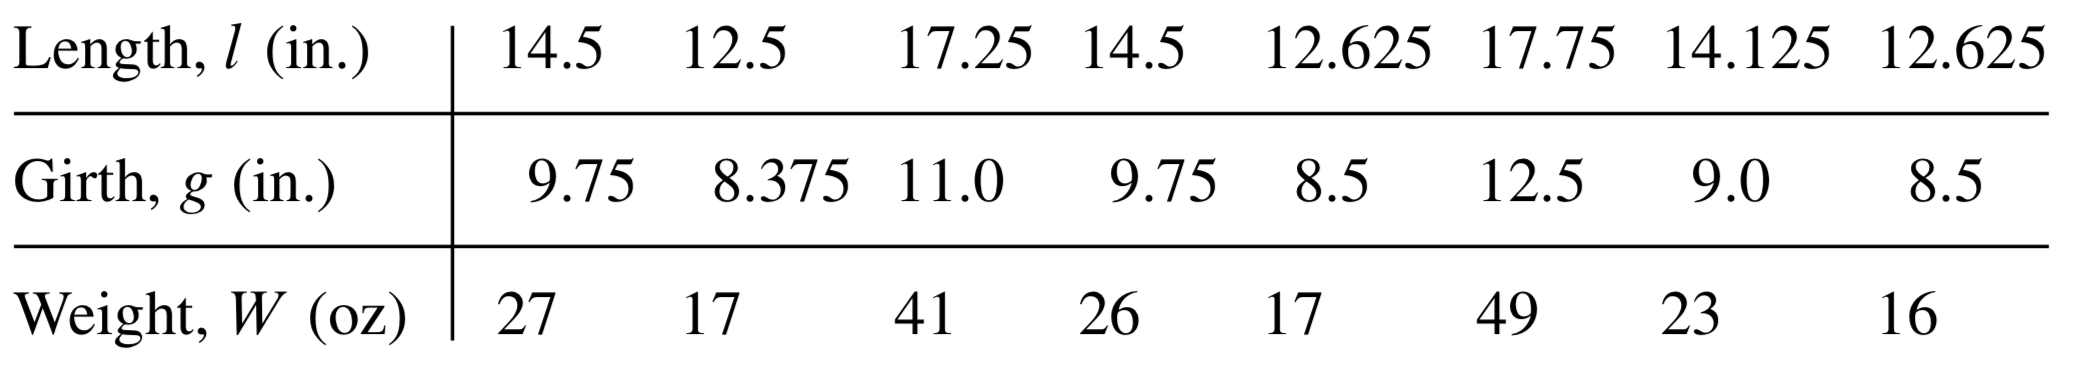
\includegraphics[width=.5\textwidth{}]{fishtab2.png}
    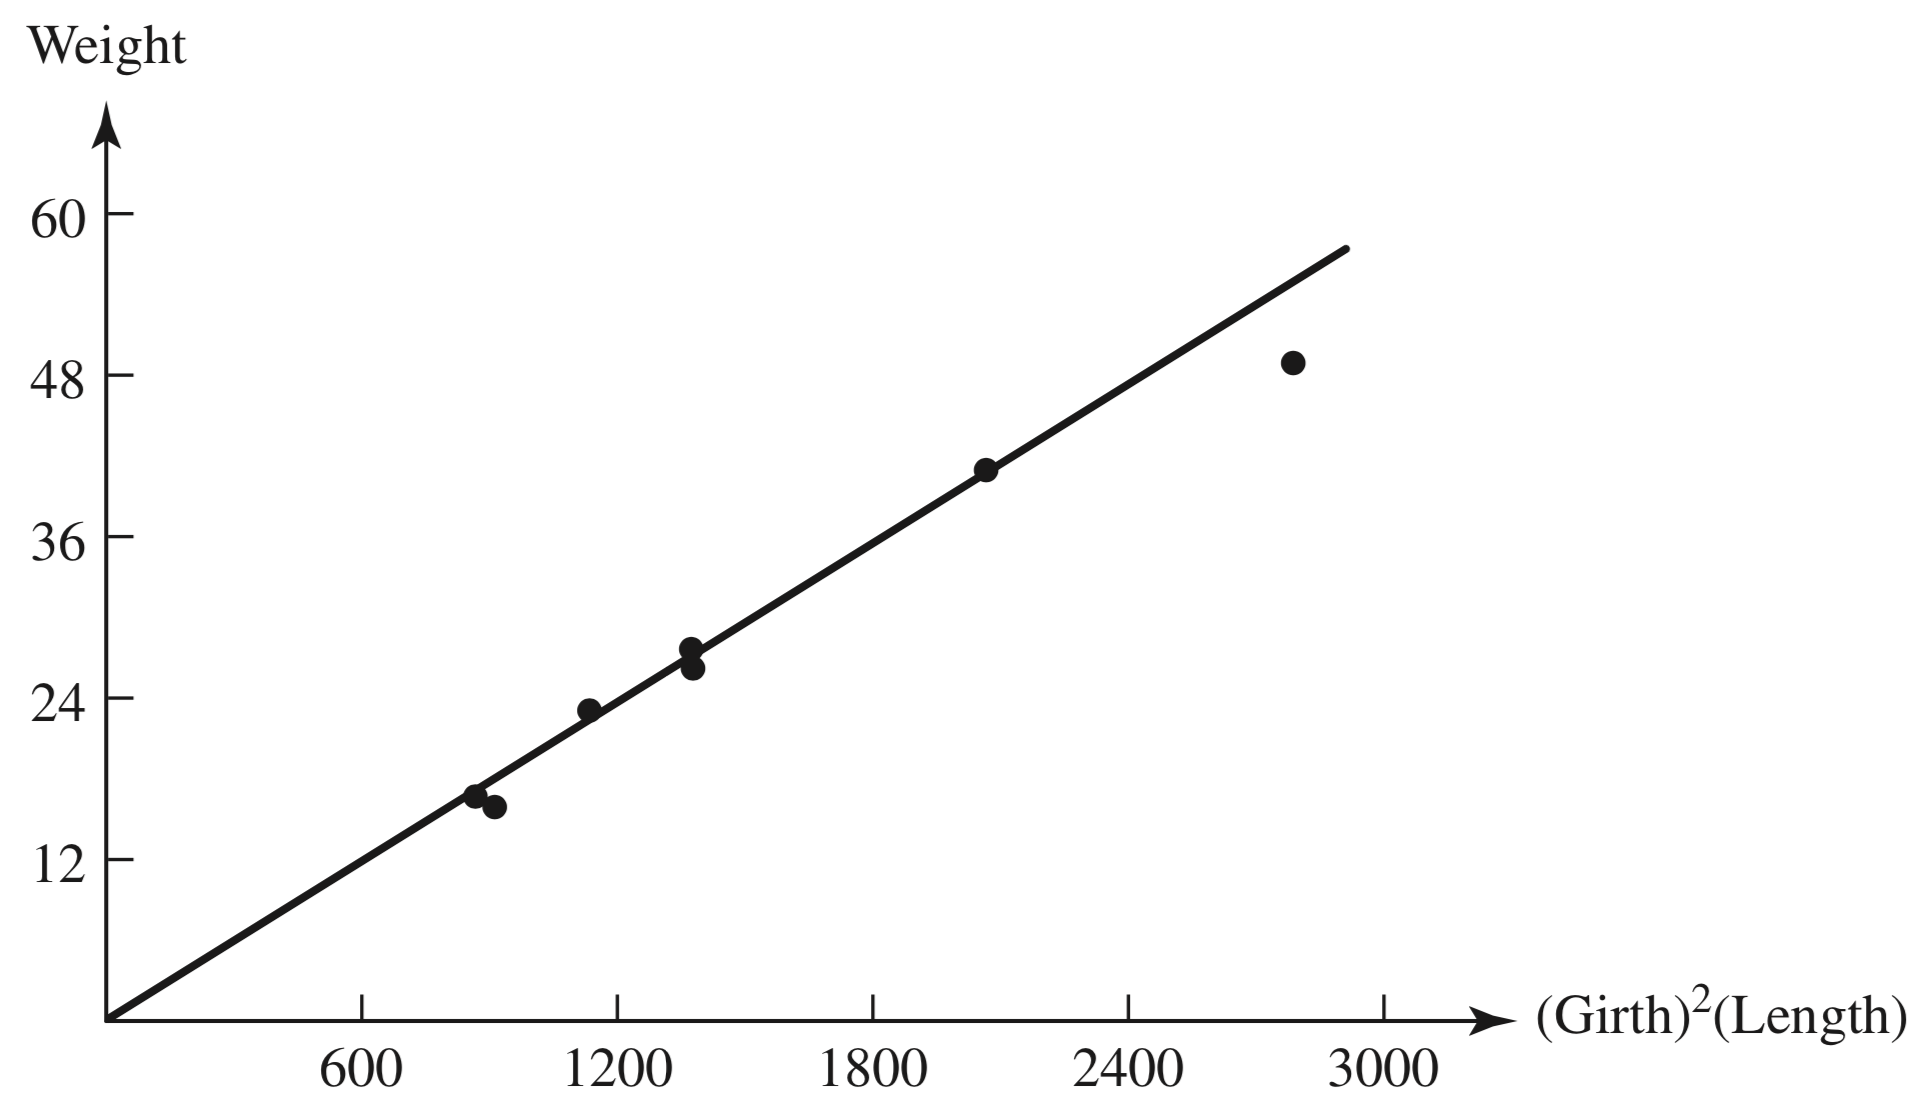
\includegraphics[width=.4\textwidth{}]{fishlen3.png}
  \end{center}
  \[
  W = 0.0196lg^2
  \]
\end{frame}

\begin{frame}{骇鸟尺寸建模}
  \begin{center}
    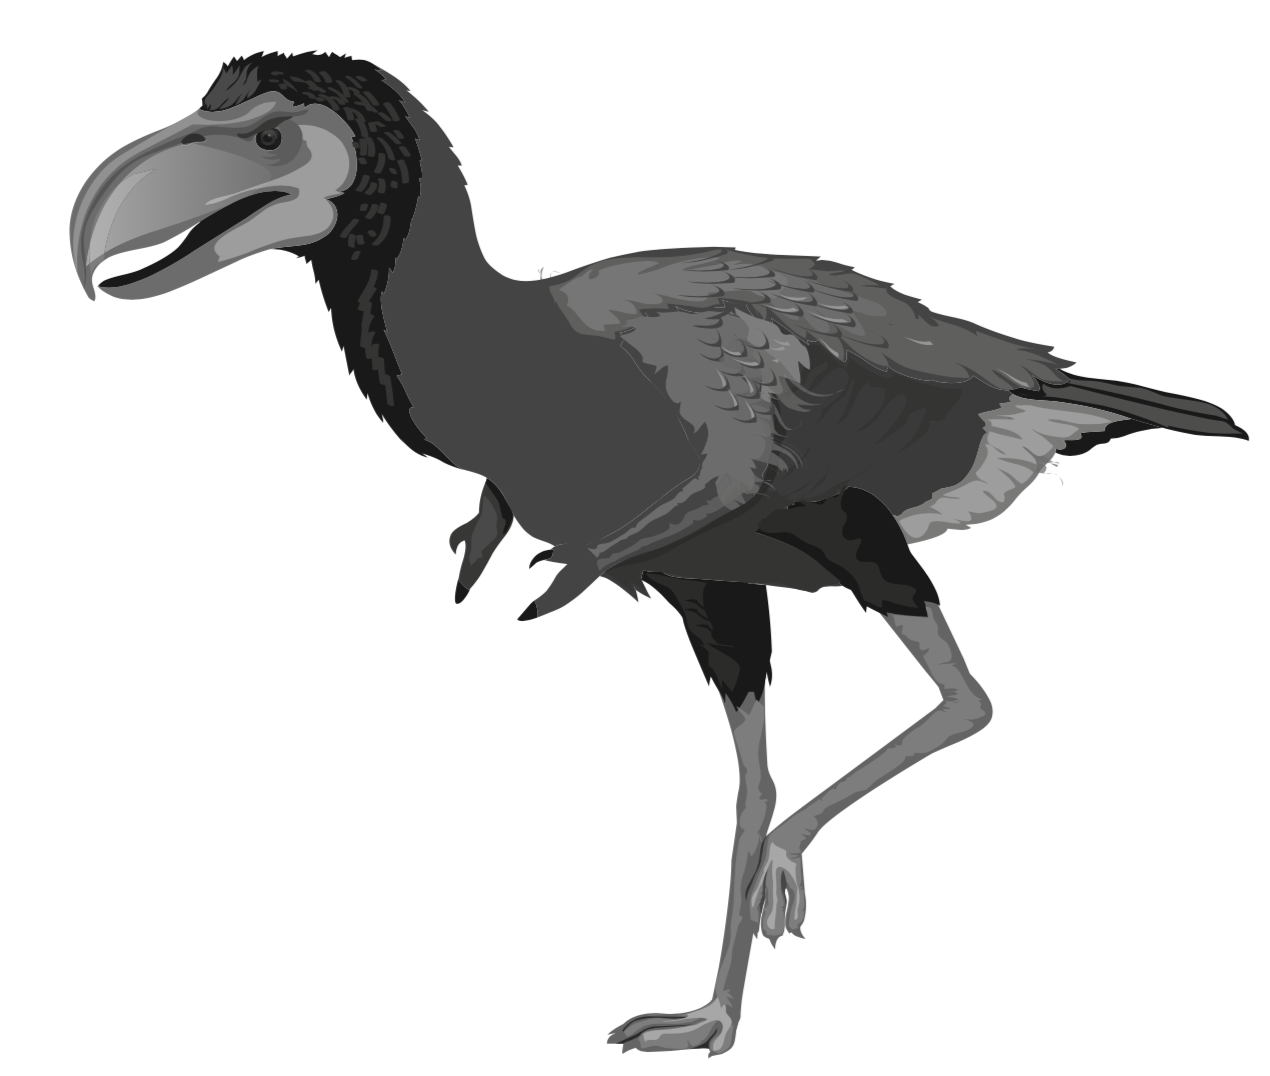
\includegraphics[width=.5\textwidth{}]{terror.png}
  \end{center}

  \begin{itemize}
  \item $W = kl^3, k>0$
  \end{itemize}

  同样的思想...
  
\end{frame}

\begin{frame}{汽车的汽油里程}
  \begin{center}
    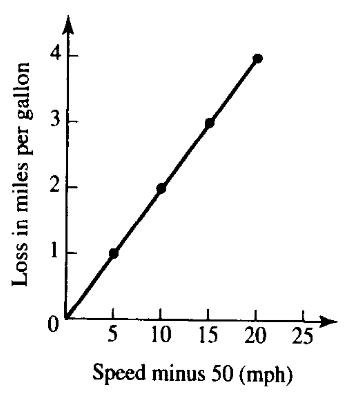
\includegraphics[width=.2\textwidth{}]{papersays.png}
  \end{center}

  \begin{description}
  \item[识别问题] 汽车的速度和它的燃油里程之间是什么关系?
  \item[假设] 燃油里程 = $f$(推进力,阻力,驾驶习惯,等等)
  \item[限制问题的识别] 忽略温度、空气密度、路况、驾驶习惯等因素
  \end{description}

\end{frame}

\begin{frame}{建模}

  \begin{itemize}
  \item 汽车常速行驶: $F_p = F_r$
  \item $K$为每加仑汽油能量,$C_r$为单位时间油耗, 则$F \propto \frac{C_rK}{v}$, 假设$K$不变, $F \propto \frac{C_r}{v}$
  \item 阻力$F_r \propto Sv^2$, 假设汽车横截面积不变$F_r \propto v^2$
  \item $F_p = F_r \Rightarrow \frac{C_rK}{v} \propto v^2 \Rightarrow C_r \propto v^3$
  \item 燃油里程 = $\frac{\text{距离}}{\text{油耗}} = \frac{vt}{C_rt}=\frac{v}{C_r}\propto v^2$
  \item 该模型可靠吗?
  \end{itemize}
  
\end{frame}

\begin{frame}{体重和身高、力量和灵活性}
  自学2.5节,思考一下:

  \begin{itemize}
  \item 一般人身高体重怎么样才合理?
  \item 为什么体操运动员身材矮小的居多?举重、短跑呢?试着去分析一下原因.
  \end{itemize}

\end{frame}

\end{document}

%%% Local Variables: 
%%% TeX-master: t
%%% TeX-engine: xetex
%%% End: 
